\begin{enumerate}[label=\thesubsection.\arabic*, ref=\thesubsection.\theenumi]
\item The line through the points $(h,   3)$ and $(4,   1)$ intersects the line $7x- 9y- 19= 0$ at a right angle. Find the value of $h$.
\label{chapters/11/10/3/10}
\\
\solution
\begin{enumerate}[label=\thesection.\arabic*.,ref=\thesection.\theenumi]
\numberwithin{equation}{enumi}
\item The equation of a line is given by 
\begin{align}
			\label{eq:app-line-school}
	y &= mx + c
	\\
	\implies \myvec{x \\ y} &= \myvec{x \\ 
	 mx + c} =\myvec{0 \\ c} + x\myvec{1 \\ m}
\end{align}
			yielding \eqref{eq:geo-param}.
\item 			\eqref{eq:app-line-school} can also be expressed as
\begin{align}
	y - mx &= c 
	\\
	\implies \myvec{-m & 1}\myvec{x \\ y} &= c
\end{align}
			yielding \eqref{eq:geo-normal}.
		\item The direction vector is 
\begin{align}
			\label{eq:app-line-school-dir}
\vec{m} = \myvec{1 \\ m}
\end{align}
and the normal vector is
\begin{align}
\vec{n}=\myvec{-m \\ 1}
			\label{eq:app-line-school-normal}
\end{align}
  \item From \eqref{eq:geo-param}, 
	  if $\vec{A},\vec{D}$ and $\vec{C}$ are on the same line,
		\label{prop:app-lin-dep}
\begin{align}
			\vec{D}=\vec{A}+q\vec{m} 
			\\ 
			\vec{C}=\vec{D}+p\vec{m} \\
			\label{eq:app-collinear} 
			\implies 	p\brak{\vec{D}-\vec{A}} 
			+ q\brak{\vec{D}-\vec{C}} = 0, \quad p, q \ne 0 \\ 
			\implies \vec{D} = \frac{p\vec{A}+q\vec{C}}{p+q} 
			\end{align} 
			yielding \eqref{eq:section_formula} upon substituting \begin{align} k = \frac{p}{q}. \end{align} 
			$\brak{\vec{D}-\vec{A}}, \brak{\vec{D}-\vec{C}}$ 
		are then said to be {\em linearly dependent}.
	\item If $\vec{A}, \vec{B}, \vec{C}$ are collinear,  from \eqref{eq:geo-normal}, \begin{align}
	 \vec{n}^{\top}\vec{A} &=  c 
	 \\
	 \vec{n}^{\top}\vec{B} &=  c 
	 \\
	 \vec{n}^{\top}\vec{C} &=  c 
\end{align}
which can be expressed as 
\begin{align}
		\label{prop:app-lin-eq}
	\myvec{ \vec{A} & \vec{B} & \vec{C}}^{\top}\vec{n} = c\myvec{1 \\ 1 \\ 1}
	\\
	\equiv \myvec{ \vec{A} & \vec{B} & \vec{C}}^{\top}\vec{n} = \myvec{1 \\ 1 \\ 1}
		\label{prop:app-lin-eq-unit-mat},
	\\
	\implies 
	\myvec{ \vec{A} & \vec{B} & \vec{C}\\ 1 & 1 &1 }^{\top}\myvec{\vec{n} \\ -1} &= \vec{0}
		\label{prop:app-lin-dep-rank}
\end{align}
yielding
		\begin{align}
			\label{eq:app-line-rank-2}
			\rank{\myvec{1 & 1 & 1 \\ \vec{A}& \vec{B}&\vec{C}}} = 2
		\end{align}
			  Rank is defined to be the number of linearly indpendent rows or columns of a matrix.
		\item
The equation of a line can also be expressed as
\begin{align}
	 \vec{n}^{\top}\vec{x} &=   1
		\label{prop:app-lin-eq-unit}
\end{align}
	  \end{enumerate}

	\item If the lines $\frac{x-1}{-3} = \frac{y-2}{2k} = \frac{z-3}{2}$ and  $\frac{x-1}{3k} = \frac{y-1}{1} = \frac{z-6}{-5}$ are perpendicular,   find the value of $k$.\\
    \solution
		\solution 
See Fig. \ref{fig:10/7/4/8Fig3}. From 
  \eqref{eq:10/7/4/8det2f}, $PQRS$ is a parallelogram.
\begin{align}
  %\label{eq:10/7/4/8det2f}
  \vec{P}  = 
 \myvec{3 \\2},\, 
 \vec{Q}  = \myvec{
 2 \\
 4 \\
 } ,\,
 \vec{R}  = \myvec{
 5 \\
 \frac{3}{2}
 }   
  ,\,
 \vec{S}  = \myvec{
 2\\
 -1 \\
 }   
 \\
	\implies 
 \brak{\vec{Q}-\vec{P}}^\top\brak{\vec{R}-\vec{Q}}  \neq 0
 \\
 \brak{\vec{R}-\vec{P}}^\top\brak{\vec{S}-\vec{Q}}  = 0
\end{align}
Therefore $PQRS$ is a rhombus.
\begin{figure}[H]
	\begin{center}
		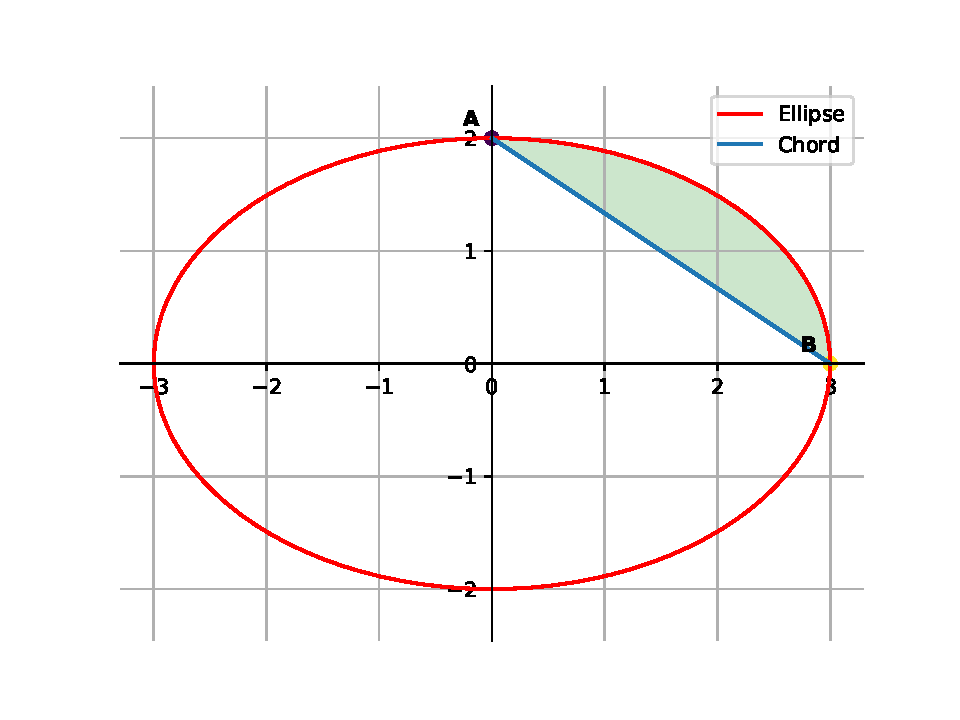
\includegraphics[width=0.75\columnwidth]{chapters/10/7/4/8/figs/fig.pdf}
	\end{center}
\caption{}
\label{fig:10/7/4/8Fig3}
\end{figure}


	\item Find the values of $\theta \text{ and } p$,  if the equation $x\cos\theta+y\sin\theta=p$ is the normal form
of the line $\sqrt{3}x+y+2=0$.
\\
\solution
		\begin{enumerate}[label=\thesection.\arabic*.,ref=\thesection.\theenumi]
\numberwithin{equation}{enumi}
\item The equation of a line is given by 
\begin{align}
			\label{eq:app-line-school}
	y &= mx + c
	\\
	\implies \myvec{x \\ y} &= \myvec{x \\ 
	 mx + c} =\myvec{0 \\ c} + x\myvec{1 \\ m}
\end{align}
			yielding \eqref{eq:geo-param}.
\item 			\eqref{eq:app-line-school} can also be expressed as
\begin{align}
	y - mx &= c 
	\\
	\implies \myvec{-m & 1}\myvec{x \\ y} &= c
\end{align}
			yielding \eqref{eq:geo-normal}.
		\item The direction vector is 
\begin{align}
			\label{eq:app-line-school-dir}
\vec{m} = \myvec{1 \\ m}
\end{align}
and the normal vector is
\begin{align}
\vec{n}=\myvec{-m \\ 1}
			\label{eq:app-line-school-normal}
\end{align}
  \item From \eqref{eq:geo-param}, 
	  if $\vec{A},\vec{D}$ and $\vec{C}$ are on the same line,
		\label{prop:app-lin-dep}
\begin{align}
			\vec{D}=\vec{A}+q\vec{m} 
			\\ 
			\vec{C}=\vec{D}+p\vec{m} \\
			\label{eq:app-collinear} 
			\implies 	p\brak{\vec{D}-\vec{A}} 
			+ q\brak{\vec{D}-\vec{C}} = 0, \quad p, q \ne 0 \\ 
			\implies \vec{D} = \frac{p\vec{A}+q\vec{C}}{p+q} 
			\end{align} 
			yielding \eqref{eq:section_formula} upon substituting \begin{align} k = \frac{p}{q}. \end{align} 
			$\brak{\vec{D}-\vec{A}}, \brak{\vec{D}-\vec{C}}$ 
		are then said to be {\em linearly dependent}.
	\item If $\vec{A}, \vec{B}, \vec{C}$ are collinear,  from \eqref{eq:geo-normal}, \begin{align}
	 \vec{n}^{\top}\vec{A} &=  c 
	 \\
	 \vec{n}^{\top}\vec{B} &=  c 
	 \\
	 \vec{n}^{\top}\vec{C} &=  c 
\end{align}
which can be expressed as 
\begin{align}
		\label{prop:app-lin-eq}
	\myvec{ \vec{A} & \vec{B} & \vec{C}}^{\top}\vec{n} = c\myvec{1 \\ 1 \\ 1}
	\\
	\equiv \myvec{ \vec{A} & \vec{B} & \vec{C}}^{\top}\vec{n} = \myvec{1 \\ 1 \\ 1}
		\label{prop:app-lin-eq-unit-mat},
	\\
	\implies 
	\myvec{ \vec{A} & \vec{B} & \vec{C}\\ 1 & 1 &1 }^{\top}\myvec{\vec{n} \\ -1} &= \vec{0}
		\label{prop:app-lin-dep-rank}
\end{align}
yielding
		\begin{align}
			\label{eq:app-line-rank-2}
			\rank{\myvec{1 & 1 & 1 \\ \vec{A}& \vec{B}&\vec{C}}} = 2
		\end{align}
			  Rank is defined to be the number of linearly indpendent rows or columns of a matrix.
		\item
The equation of a line can also be expressed as
\begin{align}
	 \vec{n}^{\top}\vec{x} &=   1
		\label{prop:app-lin-eq-unit}
\end{align}
	  \end{enumerate}

\item  Reduce the following equations into normal form. Find their perpendicular distances from the origin and angle between perpendicular and the positive $X$ axis.
\label{chapters/11/10/3/3}
\begin{enumerate}
	\item $x-\sqrt{3}y+8=0$ 
	\item $y-2=0$
	\item $x-y=4$
\end{enumerate}
\solution
\begin{enumerate}[label=\thesubsection.\arabic*, ref=\thesubsection.\theenumi]
\item Find the equation of the plane passing through the points $\brak{1, 0, -2}$,  $\brak{3, -1, 0}$ and perpendicular to the plane $2x - y + z = 8$. Also find the distance of the plane thus obtained from the origin.
\hfill (12, 2020)
    \item Find the values of $\lambda$ for which the distance of the point $(2, 1, \lambda)$ from the plane
    \begin{align}
        3x + 5y + 4z = 11
    \end{align}
    is $2\sqrt{2}$ units.
    \hfill (12, 2023)
	\item Find the distance of the point $(a, b, c)$ from the $x$-axis. \hfill (12, 2021)
	\item If the lines $\frac{x-1}{-3} = \frac{y-2}{2\lambda} = \frac{z-3}{2}$ and $\frac{x-1}{3\lambda} = \frac{y-1}{2} = \frac{z-6}{-5}$ are perpendicular, find the value of $\lambda$. Hence, determine whether the lines intersect or not. \hfill (12, 2019)
	\item Find the vector equation of the plane determined by the points $\vec{A}(3, -1, 2)$, $\vec{B}(5, 2, 4)$, and $\vec{C}(-1, -1, 6)$. Hence, find the distance of the plane, thus obtained, from the origin. \hfill (12, 2019)
	\item Find the coordinates of the foot of the perpendicular $\vec{Q}$ drawn from $\vec{P}(3, 2, 1)$ to the plane $2x - y + z + 1 = 0$. Also, find the distance $\vec{P}\vec{Q}$ and the image of the point $\vec{P}$ treating this plane as a mirror. \hfill (12, 2019)
	\item Find the value of $\lambda$ for which the following lines are perpendicular to each other:
	\begin{align*}
	\dfrac{x-5}{5(\lambda+2)} = \dfrac{2-y}{5} = \dfrac{1-z}{-1}; \quad \dfrac{x}{1} = \dfrac{y + \frac{1}{2}}{2\lambda} = \dfrac{z-1}{3}.
	\end{align*}
	Hence, find whether the lines intersect or not. \hfill (12, 2019)
	\item Find the equation of the plane passing through the point $(-1, 3, 2)$ and perpendicular to the planes $x + 2y + 3z = 5$ and $3x + 3y + z = 0$. \hfill (12, 2019)
	Gitem Find the equation of the plane passing through the point $(-1, 3, 2)$ and perpendicular to the planes $x + 2y + 3z = 5$ and $3x + 3y + z = 0$. \hfill (12, 2019)
	
	\item Find the coordinates of the foot $Q$ of the perpendicular drawn from the point $P(1, 3, 4)$ to the plane $2x - y + z + 3 = 0$. Find the distance $PQ$ and the image of $P$ treating the plane as a mirror. \hfill (12, 2019)
\item Find the coordinates of the foot of the perpendicular $\vec{Q}$ drawn from $\vec{P}(3, 2, 1)$ to the plane $2x - y + z + 1 = 0$. Also, find distance $\vec{PQ}$ and the image of the point $\vec{P}$ treating this plane as a mirror.
\hfill (12, 2018)
\item Find the vector equation of the plane determined by the points $\vec{A}\brak{3,-1,2}$, $\vec{B}\brak{5,2,4}$, $\vec{C}\brak{-1,-1,6}$. Hence, find the distance of the plane, thus obtained, from the origin.
\hfill (12, 2018)
\item Find the vector equation of the plane that contains the lines $r=\brak{\hat{i}+\hat{j}}+\lambda \brak{\hat{i}+2\hat{j} - \hat{j}}$ and the point $\brak{-1,3,-4}$. Also,find the length of the perpendicular drawn from the point $\brak{2,1,4}$ to the plane, thus obtained.
\hfill (12, 2018) 
\item Find the distance between the planes
      \begin{align*}
          \overrightarrow{r}.\myvec{2\hat{i}-3\hat{j}+6\hat{k} } - 4 =0
      \end{align*}
      and
      \begin{align*}
          \overrightarrow{r}.\myvec{6\hat{i}-9\hat{j} +18\hat{k}} +30 =0
      \end{align*}
      \hfill (12, 2016)
\item Find the position vector of the foot of perpendicular and the perpendicular distance from the point $P$ with position vector $2\hat{i}+3\hat{j}+\hat{k}$ to the plane
      \begin{align*}
          \vec{r}\cdot\brak{2\hat{i}+\hat{j}+3\hat{k}} - 26=0
      \end{align*}
      Also find image of $P$ in the plane. \hfill (12, 2016)
\item A line $l$ passes through point (-1,3,-2) and is perpendicular to both the lines $\frac {x}{1}=\frac{y}{2}=\frac{z}{3}$ and $\frac {x+2}{-3}=\frac{y-1}{2}=\frac{z+1}{5}$. Find the vector equation of the line $l$. Hence, obtain its distance from origin. \hfill (12, 2023)
\item Find the equation of the plane passing through the points $(2,1,0),(3,-2,-2)$ and $(1,1,7)$. Also, obtain its distance from the origin. \hfill (12, 2022)

\item The foot of a perpendicular drawn from the point $(-2,-1,-3)$ on a plane is $(1,-3,3)$. Find the equation of the plane. \hfill (12, 2022)
\item The distance between the planes $4x-4y+2z+5=0$ and $2x-2y+z+6=0$ is
	\begin{enumerate}
		\item $\dfrac{1}{6}$
		\item $\dfrac{7}{6}$
		\item $\dfrac{11}{6}$
		\item $\dfrac{16}{6}$
	\end{enumerate}
\hfill (12, 2022)
\item If the distance of the point $(1,1,1)$ from the plane $x-y+z+\lambda=0$ is $\dfrac{5}{\sqrt{3}}$, find the value(s) of $\lambda$. \hfill (12, 2022)

\item Find the distance of the point $(2,3,4)$ measured along the line $\dfrac{x-4}{3}=\dfrac{y+5}{6}=\dfrac{z+1}{2}$ from the plane $3x+2y+2z+5=0$. \hfill (12, 2022)

\item Find the distance of the point $P(4,3,2)$ from the plane determined by the points $A(-1,6,-5),B(-5,-2,3)$ and $C(2,4,-5)$. \hfill (12, 2022)

\item The distance of the line
	\begin{align}
		\vec{r}=(\hat{i}-\hat{j})+\lambda(\hat{i}+5\hat{j}+\hat{k})
	\end{align}
	from the plane
	\begin{align}
		\vec{r}\cdot(\hat{i}-\hat{j}+4\hat{k})=5
	\end{align}
	is
	\begin{enumerate}
		\item $\sqrt{2}$
		\item $\dfrac{1}{\sqrt{2}}$
		\item $\dfrac{1}{3\sqrt{2}}$
		\item $\dfrac{-2}{3\sqrt{2}}$
	\end{enumerate}
\hfill (12, 2022)

\item Find the values of $\lambda$, for which the distance of point $(2,1,\lambda)$ from plane $3x+5y+4z=11$ is $2\sqrt{2}$ units. \hfill (12, 2022)
\item If the distance of the point $(1,1,1)$ from the plane $x-y+z+\lambda=0$ is $\frac{5}{\sqrt{3}}$, find the value(s) of $\lambda$. \hfill (12, 2022)
\item If the line $\frac{x-1}{-3} = \frac{y-2}{2\lambda} = \frac{z-3}{2} $ and $\frac{x-1}{3\lambda} = \frac{y-1}{2}  = \frac{z-6}{-5} $ are perpendicular, find the value of $\lambda$. Hence find whether the lines are intersecting or not. \hfill (12, 2018)
\item Find the distance between the planes $2x - y + 2z = 5$ and $5x - 2.5y + 5z = 20$. \hfill (12, 2017)
\item Find the coordinates of the foot of perpendicular drawn from the point
      $A(-1, 8, 4)$ to the line joining the points $B(0, -1, 3)$ and $C(2,-3,-1)$. Hence
      find the image of the point $A$ in the line $BC$. \hfill (12, 2016)
\item The coordinates of the foot of the perpendicular drawn from the point $\brak{2,-3,4}$ on the $y-axis$ is
\hfill (12, 2020)
\item Find the equation of the plane passing through $\brak{-1,3,2}$ and perpendicular to the planes $x+2y+3z=5$ and $3x+3y+z=0$.
\hfill (12, 2018)
\item Find the equation of the plane passing through the intersection of the planes 
\begin{align*}
	\overrightarrow{\vec{r}} \cdot \brak{\hat{i} + \hat{j} + \hat{k}} &= 1
\end{align*}
and 
\begin{align*}
	\overrightarrow{\vec{r}} \cdot \brak{2\hat{i} + 3\hat{j} - \hat{k} } + 4 &= 0
\end{align*}
and parallel to the $x$-axis. Hence, find the distance of the plane from the $x$-axis. \hfill (12, 2018)
 \item Find the value of $\lambda$ for which the following lines are perpendicular to each other:
 \begin{align*}
 \dfrac{x-5}{5\lambda+2}= \dfrac{2-y}{5} = \dfrac{1-z}{-1};\dfrac{x}{1}=\dfrac{y+\dfrac{1}{2}}{2\lambda}=\dfrac{z-1}{3} 
 \end{align*}
Hence, find whether the lines intersect or not.
\hfill (12, 2018)
\item Write the equation of the line passing through $\brak{1,2,3}$ and perpendicular to the plane $\vec{r}\cdot\brak{\vec{i}+2\vec{j}-5\vec{k}}+9=0$. \hfill (12, 2015)
	\item Write the equation of a plane passing through the point $(2, 3, 7)$ and parallel to the plane obtained above. Hence, find the distance between the two parallel planes.

		\hfill (12, 2019)
	\item Find the  equation of a line passing through the point $(2, 3, 2)$ and parallel to the line $\overrightarrow{r} = (-2\hat{i} + 3\hat{j}) + \lambda (2\hat{i} - 3\hat{j} + 6\hat{k})$. Also, find the distance between these two lines.

		\hfill (12, 2019)
\end{enumerate}

\item Find the distance of the point $(-1, 1)$ from the line $12\brak{x+6} = 5\brak{y-2}$. 
\label{chapters/11/10/3/4}
	\\
\solution 
\begin{enumerate}[label=\thesection.\arabic*.,ref=\thesection.\theenumi]
\numberwithin{equation}{enumi}
\item The equation of a line is given by 
\begin{align}
			\label{eq:app-line-school}
	y &= mx + c
	\\
	\implies \myvec{x \\ y} &= \myvec{x \\ 
	 mx + c} =\myvec{0 \\ c} + x\myvec{1 \\ m}
\end{align}
			yielding \eqref{eq:geo-param}.
\item 			\eqref{eq:app-line-school} can also be expressed as
\begin{align}
	y - mx &= c 
	\\
	\implies \myvec{-m & 1}\myvec{x \\ y} &= c
\end{align}
			yielding \eqref{eq:geo-normal}.
		\item The direction vector is 
\begin{align}
			\label{eq:app-line-school-dir}
\vec{m} = \myvec{1 \\ m}
\end{align}
and the normal vector is
\begin{align}
\vec{n}=\myvec{-m \\ 1}
			\label{eq:app-line-school-normal}
\end{align}
  \item From \eqref{eq:geo-param}, 
	  if $\vec{A},\vec{D}$ and $\vec{C}$ are on the same line,
		\label{prop:app-lin-dep}
\begin{align}
			\vec{D}=\vec{A}+q\vec{m} 
			\\ 
			\vec{C}=\vec{D}+p\vec{m} \\
			\label{eq:app-collinear} 
			\implies 	p\brak{\vec{D}-\vec{A}} 
			+ q\brak{\vec{D}-\vec{C}} = 0, \quad p, q \ne 0 \\ 
			\implies \vec{D} = \frac{p\vec{A}+q\vec{C}}{p+q} 
			\end{align} 
			yielding \eqref{eq:section_formula} upon substituting \begin{align} k = \frac{p}{q}. \end{align} 
			$\brak{\vec{D}-\vec{A}}, \brak{\vec{D}-\vec{C}}$ 
		are then said to be {\em linearly dependent}.
	\item If $\vec{A}, \vec{B}, \vec{C}$ are collinear,  from \eqref{eq:geo-normal}, \begin{align}
	 \vec{n}^{\top}\vec{A} &=  c 
	 \\
	 \vec{n}^{\top}\vec{B} &=  c 
	 \\
	 \vec{n}^{\top}\vec{C} &=  c 
\end{align}
which can be expressed as 
\begin{align}
		\label{prop:app-lin-eq}
	\myvec{ \vec{A} & \vec{B} & \vec{C}}^{\top}\vec{n} = c\myvec{1 \\ 1 \\ 1}
	\\
	\equiv \myvec{ \vec{A} & \vec{B} & \vec{C}}^{\top}\vec{n} = \myvec{1 \\ 1 \\ 1}
		\label{prop:app-lin-eq-unit-mat},
	\\
	\implies 
	\myvec{ \vec{A} & \vec{B} & \vec{C}\\ 1 & 1 &1 }^{\top}\myvec{\vec{n} \\ -1} &= \vec{0}
		\label{prop:app-lin-dep-rank}
\end{align}
yielding
		\begin{align}
			\label{eq:app-line-rank-2}
			\rank{\myvec{1 & 1 & 1 \\ \vec{A}& \vec{B}&\vec{C}}} = 2
		\end{align}
			  Rank is defined to be the number of linearly indpendent rows or columns of a matrix.
		\item
The equation of a line can also be expressed as
\begin{align}
	 \vec{n}^{\top}\vec{x} &=   1
		\label{prop:app-lin-eq-unit}
\end{align}
	  \end{enumerate}

 \item  In each of the following cases,  determine the direction cosines of the normal to
the plane and the distance from the origin.
\begin{enumerate}
	\item $z=2$ 
	\item $x + y + z = 1$
	\item $2x + 3y – z = 5$
	\item $5y + 8 = 0$
\end{enumerate}
    \solution
		\input{chapters/12/11/3/1/dist.tex}
\item Find the distance between parallel lines
\label{chapters/11/10/3/6}
\begin{enumerate}
	\item $15x+8y-34=0$ and  $15x+8y+31=0$ \\
	\item  $l(x+y)+p=0$ and  $l(x+y)-r=0$
\end{enumerate}
	\solution
\input{chapters/11/10/3/6/dist.tex}
\item Find the shortest distance between the lines $l_1$ and $l_2$ whose vector equations are
\begin{align}
\overrightarrow{r}= \hat{i}+ \hat{j}+ \lambda(2 \hat{i}- \hat{j}+ \hat{k}) \\
\text{ and } \overrightarrow{r}= 2 \hat{i}+ \hat{j}- \hat{k}+ \mu(3 \hat{i}- 5 \hat{j}+ 2 \hat{k}) 
\end{align}
\item Find the points on the x-axis,  whose distances from the line $\frac{x}{3}+\frac{y}{4}=1$ are 4 units.
\label{chapters/11/10/3/5}
	\\
	\solution
\begin{enumerate}[label=\thesection.\arabic*.,ref=\thesection.\theenumi]
\numberwithin{equation}{enumi}
\item The equation of a line is given by 
\begin{align}
			\label{eq:app-line-school}
	y &= mx + c
	\\
	\implies \myvec{x \\ y} &= \myvec{x \\ 
	 mx + c} =\myvec{0 \\ c} + x\myvec{1 \\ m}
\end{align}
			yielding \eqref{eq:geo-param}.
\item 			\eqref{eq:app-line-school} can also be expressed as
\begin{align}
	y - mx &= c 
	\\
	\implies \myvec{-m & 1}\myvec{x \\ y} &= c
\end{align}
			yielding \eqref{eq:geo-normal}.
		\item The direction vector is 
\begin{align}
			\label{eq:app-line-school-dir}
\vec{m} = \myvec{1 \\ m}
\end{align}
and the normal vector is
\begin{align}
\vec{n}=\myvec{-m \\ 1}
			\label{eq:app-line-school-normal}
\end{align}
  \item From \eqref{eq:geo-param}, 
	  if $\vec{A},\vec{D}$ and $\vec{C}$ are on the same line,
		\label{prop:app-lin-dep}
\begin{align}
			\vec{D}=\vec{A}+q\vec{m} 
			\\ 
			\vec{C}=\vec{D}+p\vec{m} \\
			\label{eq:app-collinear} 
			\implies 	p\brak{\vec{D}-\vec{A}} 
			+ q\brak{\vec{D}-\vec{C}} = 0, \quad p, q \ne 0 \\ 
			\implies \vec{D} = \frac{p\vec{A}+q\vec{C}}{p+q} 
			\end{align} 
			yielding \eqref{eq:section_formula} upon substituting \begin{align} k = \frac{p}{q}. \end{align} 
			$\brak{\vec{D}-\vec{A}}, \brak{\vec{D}-\vec{C}}$ 
		are then said to be {\em linearly dependent}.
	\item If $\vec{A}, \vec{B}, \vec{C}$ are collinear,  from \eqref{eq:geo-normal}, \begin{align}
	 \vec{n}^{\top}\vec{A} &=  c 
	 \\
	 \vec{n}^{\top}\vec{B} &=  c 
	 \\
	 \vec{n}^{\top}\vec{C} &=  c 
\end{align}
which can be expressed as 
\begin{align}
		\label{prop:app-lin-eq}
	\myvec{ \vec{A} & \vec{B} & \vec{C}}^{\top}\vec{n} = c\myvec{1 \\ 1 \\ 1}
	\\
	\equiv \myvec{ \vec{A} & \vec{B} & \vec{C}}^{\top}\vec{n} = \myvec{1 \\ 1 \\ 1}
		\label{prop:app-lin-eq-unit-mat},
	\\
	\implies 
	\myvec{ \vec{A} & \vec{B} & \vec{C}\\ 1 & 1 &1 }^{\top}\myvec{\vec{n} \\ -1} &= \vec{0}
		\label{prop:app-lin-dep-rank}
\end{align}
yielding
		\begin{align}
			\label{eq:app-line-rank-2}
			\rank{\myvec{1 & 1 & 1 \\ \vec{A}& \vec{B}&\vec{C}}} = 2
		\end{align}
			  Rank is defined to be the number of linearly indpendent rows or columns of a matrix.
		\item
The equation of a line can also be expressed as
\begin{align}
	 \vec{n}^{\top}\vec{x} &=   1
		\label{prop:app-lin-eq-unit}
\end{align}
	  \end{enumerate}

\item What are the points on the y-axis whose distance from the line $\frac{x}{3}+\frac{y}{4}=1$ is 4 units.
\\
\solution
		\begin{enumerate}[label=\thesection.\arabic*.,ref=\thesection.\theenumi]
\numberwithin{equation}{enumi}
\item The equation of a line is given by 
\begin{align}
			\label{eq:app-line-school}
	y &= mx + c
	\\
	\implies \myvec{x \\ y} &= \myvec{x \\ 
	 mx + c} =\myvec{0 \\ c} + x\myvec{1 \\ m}
\end{align}
			yielding \eqref{eq:geo-param}.
\item 			\eqref{eq:app-line-school} can also be expressed as
\begin{align}
	y - mx &= c 
	\\
	\implies \myvec{-m & 1}\myvec{x \\ y} &= c
\end{align}
			yielding \eqref{eq:geo-normal}.
		\item The direction vector is 
\begin{align}
			\label{eq:app-line-school-dir}
\vec{m} = \myvec{1 \\ m}
\end{align}
and the normal vector is
\begin{align}
\vec{n}=\myvec{-m \\ 1}
			\label{eq:app-line-school-normal}
\end{align}
  \item From \eqref{eq:geo-param}, 
	  if $\vec{A},\vec{D}$ and $\vec{C}$ are on the same line,
		\label{prop:app-lin-dep}
\begin{align}
			\vec{D}=\vec{A}+q\vec{m} 
			\\ 
			\vec{C}=\vec{D}+p\vec{m} \\
			\label{eq:app-collinear} 
			\implies 	p\brak{\vec{D}-\vec{A}} 
			+ q\brak{\vec{D}-\vec{C}} = 0, \quad p, q \ne 0 \\ 
			\implies \vec{D} = \frac{p\vec{A}+q\vec{C}}{p+q} 
			\end{align} 
			yielding \eqref{eq:section_formula} upon substituting \begin{align} k = \frac{p}{q}. \end{align} 
			$\brak{\vec{D}-\vec{A}}, \brak{\vec{D}-\vec{C}}$ 
		are then said to be {\em linearly dependent}.
	\item If $\vec{A}, \vec{B}, \vec{C}$ are collinear,  from \eqref{eq:geo-normal}, \begin{align}
	 \vec{n}^{\top}\vec{A} &=  c 
	 \\
	 \vec{n}^{\top}\vec{B} &=  c 
	 \\
	 \vec{n}^{\top}\vec{C} &=  c 
\end{align}
which can be expressed as 
\begin{align}
		\label{prop:app-lin-eq}
	\myvec{ \vec{A} & \vec{B} & \vec{C}}^{\top}\vec{n} = c\myvec{1 \\ 1 \\ 1}
	\\
	\equiv \myvec{ \vec{A} & \vec{B} & \vec{C}}^{\top}\vec{n} = \myvec{1 \\ 1 \\ 1}
		\label{prop:app-lin-eq-unit-mat},
	\\
	\implies 
	\myvec{ \vec{A} & \vec{B} & \vec{C}\\ 1 & 1 &1 }^{\top}\myvec{\vec{n} \\ -1} &= \vec{0}
		\label{prop:app-lin-dep-rank}
\end{align}
yielding
		\begin{align}
			\label{eq:app-line-rank-2}
			\rank{\myvec{1 & 1 & 1 \\ \vec{A}& \vec{B}&\vec{C}}} = 2
		\end{align}
			  Rank is defined to be the number of linearly indpendent rows or columns of a matrix.
		\item
The equation of a line can also be expressed as
\begin{align}
	 \vec{n}^{\top}\vec{x} &=   1
		\label{prop:app-lin-eq-unit}
\end{align}
	  \end{enumerate}

\item Show that the path of a moving point such that its distances from two lines $3x-2y=5$ and $3x+2y=5$ are equal is a straight line.
\item Find the distance of the line $4x-y=0$ from the point $\vec{P}(4, 1)$ measured along the line making an angle of $135\degree$ with the positive x-axis.
\item Find the distance between the lines $l_1$ and $l_2$ given by
\begin{align}
\overrightarrow{r}= \hat{i}+ 2 \hat{j}- 4 \hat{k}+ \lambda(2 \hat{i}+ 3 \hat{j}+ 6 \hat{k}) \\
\text{ and }\overrightarrow{r}= 3 \hat{i}+ 3 \hat{j}- 5 \hat{k}+ \mu(2 \hat{i}+ 3 \hat{j}+ 6 \hat{k}) 
\end{align}
\item Find the distance of the plane $2x- 3y+ 4z- 6= 0$ from the origin.
\item Find the vector equation of the plane which is at a distance of $\frac{6}{\sqrt{29}}$ from the origin and its normal vector from the origin is $2 \hat{i}- 3 \hat{j}+ 4 \hat{k}$. 
\item Find the coordinates of the foot of the perpendicular from $(-1,  3)$ to the line $3x-4y-16=0$.  
\label{chapters/11/10/3/14}
\\
\solution
\begin{enumerate}[label=\thesection.\arabic*.,ref=\thesection.\theenumi]
\numberwithin{equation}{enumi}
\item The equation of a line is given by 
\begin{align}
			\label{eq:app-line-school}
	y &= mx + c
	\\
	\implies \myvec{x \\ y} &= \myvec{x \\ 
	 mx + c} =\myvec{0 \\ c} + x\myvec{1 \\ m}
\end{align}
			yielding \eqref{eq:geo-param}.
\item 			\eqref{eq:app-line-school} can also be expressed as
\begin{align}
	y - mx &= c 
	\\
	\implies \myvec{-m & 1}\myvec{x \\ y} &= c
\end{align}
			yielding \eqref{eq:geo-normal}.
		\item The direction vector is 
\begin{align}
			\label{eq:app-line-school-dir}
\vec{m} = \myvec{1 \\ m}
\end{align}
and the normal vector is
\begin{align}
\vec{n}=\myvec{-m \\ 1}
			\label{eq:app-line-school-normal}
\end{align}
  \item From \eqref{eq:geo-param}, 
	  if $\vec{A},\vec{D}$ and $\vec{C}$ are on the same line,
		\label{prop:app-lin-dep}
\begin{align}
			\vec{D}=\vec{A}+q\vec{m} 
			\\ 
			\vec{C}=\vec{D}+p\vec{m} \\
			\label{eq:app-collinear} 
			\implies 	p\brak{\vec{D}-\vec{A}} 
			+ q\brak{\vec{D}-\vec{C}} = 0, \quad p, q \ne 0 \\ 
			\implies \vec{D} = \frac{p\vec{A}+q\vec{C}}{p+q} 
			\end{align} 
			yielding \eqref{eq:section_formula} upon substituting \begin{align} k = \frac{p}{q}. \end{align} 
			$\brak{\vec{D}-\vec{A}}, \brak{\vec{D}-\vec{C}}$ 
		are then said to be {\em linearly dependent}.
	\item If $\vec{A}, \vec{B}, \vec{C}$ are collinear,  from \eqref{eq:geo-normal}, \begin{align}
	 \vec{n}^{\top}\vec{A} &=  c 
	 \\
	 \vec{n}^{\top}\vec{B} &=  c 
	 \\
	 \vec{n}^{\top}\vec{C} &=  c 
\end{align}
which can be expressed as 
\begin{align}
		\label{prop:app-lin-eq}
	\myvec{ \vec{A} & \vec{B} & \vec{C}}^{\top}\vec{n} = c\myvec{1 \\ 1 \\ 1}
	\\
	\equiv \myvec{ \vec{A} & \vec{B} & \vec{C}}^{\top}\vec{n} = \myvec{1 \\ 1 \\ 1}
		\label{prop:app-lin-eq-unit-mat},
	\\
	\implies 
	\myvec{ \vec{A} & \vec{B} & \vec{C}\\ 1 & 1 &1 }^{\top}\myvec{\vec{n} \\ -1} &= \vec{0}
		\label{prop:app-lin-dep-rank}
\end{align}
yielding
		\begin{align}
			\label{eq:app-line-rank-2}
			\rank{\myvec{1 & 1 & 1 \\ \vec{A}& \vec{B}&\vec{C}}} = 2
		\end{align}
			  Rank is defined to be the number of linearly indpendent rows or columns of a matrix.
		\item
The equation of a line can also be expressed as
\begin{align}
	 \vec{n}^{\top}\vec{x} &=   1
		\label{prop:app-lin-eq-unit}
\end{align}
	  \end{enumerate}

\item Find the equation of a line whose perpendicular distance from the origin is 5 units and the angle made by the perpendicular with the positive $X$ axis is $30\degree$.
\label{chapters/11/10/2/8}
\\
\solution
\begin{enumerate}[label=\thesection.\arabic*.,ref=\thesection.\theenumi]
\numberwithin{equation}{enumi}
\item The equation of a line is given by 
\begin{align}
			\label{eq:app-line-school}
	y &= mx + c
	\\
	\implies \myvec{x \\ y} &= \myvec{x \\ 
	 mx + c} =\myvec{0 \\ c} + x\myvec{1 \\ m}
\end{align}
			yielding \eqref{eq:geo-param}.
\item 			\eqref{eq:app-line-school} can also be expressed as
\begin{align}
	y - mx &= c 
	\\
	\implies \myvec{-m & 1}\myvec{x \\ y} &= c
\end{align}
			yielding \eqref{eq:geo-normal}.
		\item The direction vector is 
\begin{align}
			\label{eq:app-line-school-dir}
\vec{m} = \myvec{1 \\ m}
\end{align}
and the normal vector is
\begin{align}
\vec{n}=\myvec{-m \\ 1}
			\label{eq:app-line-school-normal}
\end{align}
  \item From \eqref{eq:geo-param}, 
	  if $\vec{A},\vec{D}$ and $\vec{C}$ are on the same line,
		\label{prop:app-lin-dep}
\begin{align}
			\vec{D}=\vec{A}+q\vec{m} 
			\\ 
			\vec{C}=\vec{D}+p\vec{m} \\
			\label{eq:app-collinear} 
			\implies 	p\brak{\vec{D}-\vec{A}} 
			+ q\brak{\vec{D}-\vec{C}} = 0, \quad p, q \ne 0 \\ 
			\implies \vec{D} = \frac{p\vec{A}+q\vec{C}}{p+q} 
			\end{align} 
			yielding \eqref{eq:section_formula} upon substituting \begin{align} k = \frac{p}{q}. \end{align} 
			$\brak{\vec{D}-\vec{A}}, \brak{\vec{D}-\vec{C}}$ 
		are then said to be {\em linearly dependent}.
	\item If $\vec{A}, \vec{B}, \vec{C}$ are collinear,  from \eqref{eq:geo-normal}, \begin{align}
	 \vec{n}^{\top}\vec{A} &=  c 
	 \\
	 \vec{n}^{\top}\vec{B} &=  c 
	 \\
	 \vec{n}^{\top}\vec{C} &=  c 
\end{align}
which can be expressed as 
\begin{align}
		\label{prop:app-lin-eq}
	\myvec{ \vec{A} & \vec{B} & \vec{C}}^{\top}\vec{n} = c\myvec{1 \\ 1 \\ 1}
	\\
	\equiv \myvec{ \vec{A} & \vec{B} & \vec{C}}^{\top}\vec{n} = \myvec{1 \\ 1 \\ 1}
		\label{prop:app-lin-eq-unit-mat},
	\\
	\implies 
	\myvec{ \vec{A} & \vec{B} & \vec{C}\\ 1 & 1 &1 }^{\top}\myvec{\vec{n} \\ -1} &= \vec{0}
		\label{prop:app-lin-dep-rank}
\end{align}
yielding
		\begin{align}
			\label{eq:app-line-rank-2}
			\rank{\myvec{1 & 1 & 1 \\ \vec{A}& \vec{B}&\vec{C}}} = 2
		\end{align}
			  Rank is defined to be the number of linearly indpendent rows or columns of a matrix.
		\item
The equation of a line can also be expressed as
\begin{align}
	 \vec{n}^{\top}\vec{x} &=   1
		\label{prop:app-lin-eq-unit}
\end{align}
	  \end{enumerate}

\item In the triangle $ABC$ with vertices $\vec{A} \brak{2,  3}$,  $\vec{B} \brak{4,  –1}$ and $\vec{C} \brak{1,  2}$,  find the equation and length of altitude from the vertex $\vec{A}$.
\label{chapters/11/10/3/17}
\\
\solution
\begin{enumerate}[label=\thesection.\arabic*.,ref=\thesection.\theenumi]
\numberwithin{equation}{enumi}
\item The equation of a line is given by 
\begin{align}
			\label{eq:app-line-school}
	y &= mx + c
	\\
	\implies \myvec{x \\ y} &= \myvec{x \\ 
	 mx + c} =\myvec{0 \\ c} + x\myvec{1 \\ m}
\end{align}
			yielding \eqref{eq:geo-param}.
\item 			\eqref{eq:app-line-school} can also be expressed as
\begin{align}
	y - mx &= c 
	\\
	\implies \myvec{-m & 1}\myvec{x \\ y} &= c
\end{align}
			yielding \eqref{eq:geo-normal}.
		\item The direction vector is 
\begin{align}
			\label{eq:app-line-school-dir}
\vec{m} = \myvec{1 \\ m}
\end{align}
and the normal vector is
\begin{align}
\vec{n}=\myvec{-m \\ 1}
			\label{eq:app-line-school-normal}
\end{align}
  \item From \eqref{eq:geo-param}, 
	  if $\vec{A},\vec{D}$ and $\vec{C}$ are on the same line,
		\label{prop:app-lin-dep}
\begin{align}
			\vec{D}=\vec{A}+q\vec{m} 
			\\ 
			\vec{C}=\vec{D}+p\vec{m} \\
			\label{eq:app-collinear} 
			\implies 	p\brak{\vec{D}-\vec{A}} 
			+ q\brak{\vec{D}-\vec{C}} = 0, \quad p, q \ne 0 \\ 
			\implies \vec{D} = \frac{p\vec{A}+q\vec{C}}{p+q} 
			\end{align} 
			yielding \eqref{eq:section_formula} upon substituting \begin{align} k = \frac{p}{q}. \end{align} 
			$\brak{\vec{D}-\vec{A}}, \brak{\vec{D}-\vec{C}}$ 
		are then said to be {\em linearly dependent}.
	\item If $\vec{A}, \vec{B}, \vec{C}$ are collinear,  from \eqref{eq:geo-normal}, \begin{align}
	 \vec{n}^{\top}\vec{A} &=  c 
	 \\
	 \vec{n}^{\top}\vec{B} &=  c 
	 \\
	 \vec{n}^{\top}\vec{C} &=  c 
\end{align}
which can be expressed as 
\begin{align}
		\label{prop:app-lin-eq}
	\myvec{ \vec{A} & \vec{B} & \vec{C}}^{\top}\vec{n} = c\myvec{1 \\ 1 \\ 1}
	\\
	\equiv \myvec{ \vec{A} & \vec{B} & \vec{C}}^{\top}\vec{n} = \myvec{1 \\ 1 \\ 1}
		\label{prop:app-lin-eq-unit-mat},
	\\
	\implies 
	\myvec{ \vec{A} & \vec{B} & \vec{C}\\ 1 & 1 &1 }^{\top}\myvec{\vec{n} \\ -1} &= \vec{0}
		\label{prop:app-lin-dep-rank}
\end{align}
yielding
		\begin{align}
			\label{eq:app-line-rank-2}
			\rank{\myvec{1 & 1 & 1 \\ \vec{A}& \vec{B}&\vec{C}}} = 2
		\end{align}
			  Rank is defined to be the number of linearly indpendent rows or columns of a matrix.
		\item
The equation of a line can also be expressed as
\begin{align}
	 \vec{n}^{\top}\vec{x} &=   1
		\label{prop:app-lin-eq-unit}
\end{align}
	  \end{enumerate}

\item Find the equation of a line  drawn perpendicular to the line $\frac{x}{4}+\frac{y}{6}=1$ through the point where it meets the y-axis. \\
\solution
		\begin{enumerate}[label=\thesection.\arabic*.,ref=\thesection.\theenumi]
\numberwithin{equation}{enumi}
\item The equation of a line is given by 
\begin{align}
			\label{eq:app-line-school}
	y &= mx + c
	\\
	\implies \myvec{x \\ y} &= \myvec{x \\ 
	 mx + c} =\myvec{0 \\ c} + x\myvec{1 \\ m}
\end{align}
			yielding \eqref{eq:geo-param}.
\item 			\eqref{eq:app-line-school} can also be expressed as
\begin{align}
	y - mx &= c 
	\\
	\implies \myvec{-m & 1}\myvec{x \\ y} &= c
\end{align}
			yielding \eqref{eq:geo-normal}.
		\item The direction vector is 
\begin{align}
			\label{eq:app-line-school-dir}
\vec{m} = \myvec{1 \\ m}
\end{align}
and the normal vector is
\begin{align}
\vec{n}=\myvec{-m \\ 1}
			\label{eq:app-line-school-normal}
\end{align}
  \item From \eqref{eq:geo-param}, 
	  if $\vec{A},\vec{D}$ and $\vec{C}$ are on the same line,
		\label{prop:app-lin-dep}
\begin{align}
			\vec{D}=\vec{A}+q\vec{m} 
			\\ 
			\vec{C}=\vec{D}+p\vec{m} \\
			\label{eq:app-collinear} 
			\implies 	p\brak{\vec{D}-\vec{A}} 
			+ q\brak{\vec{D}-\vec{C}} = 0, \quad p, q \ne 0 \\ 
			\implies \vec{D} = \frac{p\vec{A}+q\vec{C}}{p+q} 
			\end{align} 
			yielding \eqref{eq:section_formula} upon substituting \begin{align} k = \frac{p}{q}. \end{align} 
			$\brak{\vec{D}-\vec{A}}, \brak{\vec{D}-\vec{C}}$ 
		are then said to be {\em linearly dependent}.
	\item If $\vec{A}, \vec{B}, \vec{C}$ are collinear,  from \eqref{eq:geo-normal}, \begin{align}
	 \vec{n}^{\top}\vec{A} &=  c 
	 \\
	 \vec{n}^{\top}\vec{B} &=  c 
	 \\
	 \vec{n}^{\top}\vec{C} &=  c 
\end{align}
which can be expressed as 
\begin{align}
		\label{prop:app-lin-eq}
	\myvec{ \vec{A} & \vec{B} & \vec{C}}^{\top}\vec{n} = c\myvec{1 \\ 1 \\ 1}
	\\
	\equiv \myvec{ \vec{A} & \vec{B} & \vec{C}}^{\top}\vec{n} = \myvec{1 \\ 1 \\ 1}
		\label{prop:app-lin-eq-unit-mat},
	\\
	\implies 
	\myvec{ \vec{A} & \vec{B} & \vec{C}\\ 1 & 1 &1 }^{\top}\myvec{\vec{n} \\ -1} &= \vec{0}
		\label{prop:app-lin-dep-rank}
\end{align}
yielding
		\begin{align}
			\label{eq:app-line-rank-2}
			\rank{\myvec{1 & 1 & 1 \\ \vec{A}& \vec{B}&\vec{C}}} = 2
		\end{align}
			  Rank is defined to be the number of linearly indpendent rows or columns of a matrix.
		\item
The equation of a line can also be expressed as
\begin{align}
	 \vec{n}^{\top}\vec{x} &=   1
		\label{prop:app-lin-eq-unit}
\end{align}
	  \end{enumerate}

\item Find the equation of line perpendicular to the line $x-7y+5=0$ and having $x$ intercept $3$.\\
\label{chapters/11/10/3/8}
\solution
\begin{enumerate}[label=\thesection.\arabic*.,ref=\thesection.\theenumi]
\numberwithin{equation}{enumi}
\item The equation of a line is given by 
\begin{align}
			\label{eq:app-line-school}
	y &= mx + c
	\\
	\implies \myvec{x \\ y} &= \myvec{x \\ 
	 mx + c} =\myvec{0 \\ c} + x\myvec{1 \\ m}
\end{align}
			yielding \eqref{eq:geo-param}.
\item 			\eqref{eq:app-line-school} can also be expressed as
\begin{align}
	y - mx &= c 
	\\
	\implies \myvec{-m & 1}\myvec{x \\ y} &= c
\end{align}
			yielding \eqref{eq:geo-normal}.
		\item The direction vector is 
\begin{align}
			\label{eq:app-line-school-dir}
\vec{m} = \myvec{1 \\ m}
\end{align}
and the normal vector is
\begin{align}
\vec{n}=\myvec{-m \\ 1}
			\label{eq:app-line-school-normal}
\end{align}
  \item From \eqref{eq:geo-param}, 
	  if $\vec{A},\vec{D}$ and $\vec{C}$ are on the same line,
		\label{prop:app-lin-dep}
\begin{align}
			\vec{D}=\vec{A}+q\vec{m} 
			\\ 
			\vec{C}=\vec{D}+p\vec{m} \\
			\label{eq:app-collinear} 
			\implies 	p\brak{\vec{D}-\vec{A}} 
			+ q\brak{\vec{D}-\vec{C}} = 0, \quad p, q \ne 0 \\ 
			\implies \vec{D} = \frac{p\vec{A}+q\vec{C}}{p+q} 
			\end{align} 
			yielding \eqref{eq:section_formula} upon substituting \begin{align} k = \frac{p}{q}. \end{align} 
			$\brak{\vec{D}-\vec{A}}, \brak{\vec{D}-\vec{C}}$ 
		are then said to be {\em linearly dependent}.
	\item If $\vec{A}, \vec{B}, \vec{C}$ are collinear,  from \eqref{eq:geo-normal}, \begin{align}
	 \vec{n}^{\top}\vec{A} &=  c 
	 \\
	 \vec{n}^{\top}\vec{B} &=  c 
	 \\
	 \vec{n}^{\top}\vec{C} &=  c 
\end{align}
which can be expressed as 
\begin{align}
		\label{prop:app-lin-eq}
	\myvec{ \vec{A} & \vec{B} & \vec{C}}^{\top}\vec{n} = c\myvec{1 \\ 1 \\ 1}
	\\
	\equiv \myvec{ \vec{A} & \vec{B} & \vec{C}}^{\top}\vec{n} = \myvec{1 \\ 1 \\ 1}
		\label{prop:app-lin-eq-unit-mat},
	\\
	\implies 
	\myvec{ \vec{A} & \vec{B} & \vec{C}\\ 1 & 1 &1 }^{\top}\myvec{\vec{n} \\ -1} &= \vec{0}
		\label{prop:app-lin-dep-rank}
\end{align}
yielding
		\begin{align}
			\label{eq:app-line-rank-2}
			\rank{\myvec{1 & 1 & 1 \\ \vec{A}& \vec{B}&\vec{C}}} = 2
		\end{align}
			  Rank is defined to be the number of linearly indpendent rows or columns of a matrix.
		\item
The equation of a line can also be expressed as
\begin{align}
	 \vec{n}^{\top}\vec{x} &=   1
		\label{prop:app-lin-eq-unit}
\end{align}
	  \end{enumerate}

\item Find the equation of one of the sides of an isosceles right angled triangle whose hypotenuse is given by $3x+4y=4$ and the opposite vertex of the hypotenuse is (2, 2).
\item In what direction should a line be drawn through the point (1, 2) so that its point of intersection with line $x+y=4$ is at a distance $\sqrt{6}{3}$. 
\item Find the equation of a line which is equidistant from parallel lines $9x+6y-7=0$ and $3x+2y+6=0$.
\\
\solution
		\begin{enumerate}[label=\thesection.\arabic*.,ref=\thesection.\theenumi]
\numberwithin{equation}{enumi}
\item The equation of a line is given by 
\begin{align}
			\label{eq:app-line-school}
	y &= mx + c
	\\
	\implies \myvec{x \\ y} &= \myvec{x \\ 
	 mx + c} =\myvec{0 \\ c} + x\myvec{1 \\ m}
\end{align}
			yielding \eqref{eq:geo-param}.
\item 			\eqref{eq:app-line-school} can also be expressed as
\begin{align}
	y - mx &= c 
	\\
	\implies \myvec{-m & 1}\myvec{x \\ y} &= c
\end{align}
			yielding \eqref{eq:geo-normal}.
		\item The direction vector is 
\begin{align}
			\label{eq:app-line-school-dir}
\vec{m} = \myvec{1 \\ m}
\end{align}
and the normal vector is
\begin{align}
\vec{n}=\myvec{-m \\ 1}
			\label{eq:app-line-school-normal}
\end{align}
  \item From \eqref{eq:geo-param}, 
	  if $\vec{A},\vec{D}$ and $\vec{C}$ are on the same line,
		\label{prop:app-lin-dep}
\begin{align}
			\vec{D}=\vec{A}+q\vec{m} 
			\\ 
			\vec{C}=\vec{D}+p\vec{m} \\
			\label{eq:app-collinear} 
			\implies 	p\brak{\vec{D}-\vec{A}} 
			+ q\brak{\vec{D}-\vec{C}} = 0, \quad p, q \ne 0 \\ 
			\implies \vec{D} = \frac{p\vec{A}+q\vec{C}}{p+q} 
			\end{align} 
			yielding \eqref{eq:section_formula} upon substituting \begin{align} k = \frac{p}{q}. \end{align} 
			$\brak{\vec{D}-\vec{A}}, \brak{\vec{D}-\vec{C}}$ 
		are then said to be {\em linearly dependent}.
	\item If $\vec{A}, \vec{B}, \vec{C}$ are collinear,  from \eqref{eq:geo-normal}, \begin{align}
	 \vec{n}^{\top}\vec{A} &=  c 
	 \\
	 \vec{n}^{\top}\vec{B} &=  c 
	 \\
	 \vec{n}^{\top}\vec{C} &=  c 
\end{align}
which can be expressed as 
\begin{align}
		\label{prop:app-lin-eq}
	\myvec{ \vec{A} & \vec{B} & \vec{C}}^{\top}\vec{n} = c\myvec{1 \\ 1 \\ 1}
	\\
	\equiv \myvec{ \vec{A} & \vec{B} & \vec{C}}^{\top}\vec{n} = \myvec{1 \\ 1 \\ 1}
		\label{prop:app-lin-eq-unit-mat},
	\\
	\implies 
	\myvec{ \vec{A} & \vec{B} & \vec{C}\\ 1 & 1 &1 }^{\top}\myvec{\vec{n} \\ -1} &= \vec{0}
		\label{prop:app-lin-dep-rank}
\end{align}
yielding
		\begin{align}
			\label{eq:app-line-rank-2}
			\rank{\myvec{1 & 1 & 1 \\ \vec{A}& \vec{B}&\vec{C}}} = 2
		\end{align}
			  Rank is defined to be the number of linearly indpendent rows or columns of a matrix.
		\item
The equation of a line can also be expressed as
\begin{align}
	 \vec{n}^{\top}\vec{x} &=   1
		\label{prop:app-lin-eq-unit}
\end{align}
	  \end{enumerate}

\item Find the equation of the line passing through the point (5, 2) and perpendicular to the line joining the points (2, 3) and (3,  -1).
\item Find the points on the line $x+y=4$ which lie at a unit distance from the line $4x+3y=10$.
\item Find the equation of a straight line on which length of perpendicular from the origin is four units and the line makes on angle of 120$\degree$ with the positive direction of $X$ axis. 
\item The equation of the straight line passing through the point (3, 2) and perpendicular to the line $y=x$ is \rule{1cm}{0.1pt}.
\item 
	Find the equation of the line passing through  (-3, 5) and perpendicular to the line through the points (2, 5) and (-3, 6).
	\\
	\solution 
\label{chapters/11/10/2/10}
\begin{enumerate}[label=\thesection.\arabic*.,ref=\thesection.\theenumi]
\numberwithin{equation}{enumi}
\item The equation of a line is given by 
\begin{align}
			\label{eq:app-line-school}
	y &= mx + c
	\\
	\implies \myvec{x \\ y} &= \myvec{x \\ 
	 mx + c} =\myvec{0 \\ c} + x\myvec{1 \\ m}
\end{align}
			yielding \eqref{eq:geo-param}.
\item 			\eqref{eq:app-line-school} can also be expressed as
\begin{align}
	y - mx &= c 
	\\
	\implies \myvec{-m & 1}\myvec{x \\ y} &= c
\end{align}
			yielding \eqref{eq:geo-normal}.
		\item The direction vector is 
\begin{align}
			\label{eq:app-line-school-dir}
\vec{m} = \myvec{1 \\ m}
\end{align}
and the normal vector is
\begin{align}
\vec{n}=\myvec{-m \\ 1}
			\label{eq:app-line-school-normal}
\end{align}
  \item From \eqref{eq:geo-param}, 
	  if $\vec{A},\vec{D}$ and $\vec{C}$ are on the same line,
		\label{prop:app-lin-dep}
\begin{align}
			\vec{D}=\vec{A}+q\vec{m} 
			\\ 
			\vec{C}=\vec{D}+p\vec{m} \\
			\label{eq:app-collinear} 
			\implies 	p\brak{\vec{D}-\vec{A}} 
			+ q\brak{\vec{D}-\vec{C}} = 0, \quad p, q \ne 0 \\ 
			\implies \vec{D} = \frac{p\vec{A}+q\vec{C}}{p+q} 
			\end{align} 
			yielding \eqref{eq:section_formula} upon substituting \begin{align} k = \frac{p}{q}. \end{align} 
			$\brak{\vec{D}-\vec{A}}, \brak{\vec{D}-\vec{C}}$ 
		are then said to be {\em linearly dependent}.
	\item If $\vec{A}, \vec{B}, \vec{C}$ are collinear,  from \eqref{eq:geo-normal}, \begin{align}
	 \vec{n}^{\top}\vec{A} &=  c 
	 \\
	 \vec{n}^{\top}\vec{B} &=  c 
	 \\
	 \vec{n}^{\top}\vec{C} &=  c 
\end{align}
which can be expressed as 
\begin{align}
		\label{prop:app-lin-eq}
	\myvec{ \vec{A} & \vec{B} & \vec{C}}^{\top}\vec{n} = c\myvec{1 \\ 1 \\ 1}
	\\
	\equiv \myvec{ \vec{A} & \vec{B} & \vec{C}}^{\top}\vec{n} = \myvec{1 \\ 1 \\ 1}
		\label{prop:app-lin-eq-unit-mat},
	\\
	\implies 
	\myvec{ \vec{A} & \vec{B} & \vec{C}\\ 1 & 1 &1 }^{\top}\myvec{\vec{n} \\ -1} &= \vec{0}
		\label{prop:app-lin-dep-rank}
\end{align}
yielding
		\begin{align}
			\label{eq:app-line-rank-2}
			\rank{\myvec{1 & 1 & 1 \\ \vec{A}& \vec{B}&\vec{C}}} = 2
		\end{align}
			  Rank is defined to be the number of linearly indpendent rows or columns of a matrix.
		\item
The equation of a line can also be expressed as
\begin{align}
	 \vec{n}^{\top}\vec{x} &=   1
		\label{prop:app-lin-eq-unit}
\end{align}
	  \end{enumerate}

\item 
	The perpendicular from the origin to a line meets it at the point $(-2, 9)$. Find the equation of the line.
\label{chapters/11/10/2/15}
	\\
	\solution
\begin{enumerate}[label=\thesection.\arabic*.,ref=\thesection.\theenumi]
\numberwithin{equation}{enumi}
\item The equation of a line is given by 
\begin{align}
			\label{eq:app-line-school}
	y &= mx + c
	\\
	\implies \myvec{x \\ y} &= \myvec{x \\ 
	 mx + c} =\myvec{0 \\ c} + x\myvec{1 \\ m}
\end{align}
			yielding \eqref{eq:geo-param}.
\item 			\eqref{eq:app-line-school} can also be expressed as
\begin{align}
	y - mx &= c 
	\\
	\implies \myvec{-m & 1}\myvec{x \\ y} &= c
\end{align}
			yielding \eqref{eq:geo-normal}.
		\item The direction vector is 
\begin{align}
			\label{eq:app-line-school-dir}
\vec{m} = \myvec{1 \\ m}
\end{align}
and the normal vector is
\begin{align}
\vec{n}=\myvec{-m \\ 1}
			\label{eq:app-line-school-normal}
\end{align}
  \item From \eqref{eq:geo-param}, 
	  if $\vec{A},\vec{D}$ and $\vec{C}$ are on the same line,
		\label{prop:app-lin-dep}
\begin{align}
			\vec{D}=\vec{A}+q\vec{m} 
			\\ 
			\vec{C}=\vec{D}+p\vec{m} \\
			\label{eq:app-collinear} 
			\implies 	p\brak{\vec{D}-\vec{A}} 
			+ q\brak{\vec{D}-\vec{C}} = 0, \quad p, q \ne 0 \\ 
			\implies \vec{D} = \frac{p\vec{A}+q\vec{C}}{p+q} 
			\end{align} 
			yielding \eqref{eq:section_formula} upon substituting \begin{align} k = \frac{p}{q}. \end{align} 
			$\brak{\vec{D}-\vec{A}}, \brak{\vec{D}-\vec{C}}$ 
		are then said to be {\em linearly dependent}.
	\item If $\vec{A}, \vec{B}, \vec{C}$ are collinear,  from \eqref{eq:geo-normal}, \begin{align}
	 \vec{n}^{\top}\vec{A} &=  c 
	 \\
	 \vec{n}^{\top}\vec{B} &=  c 
	 \\
	 \vec{n}^{\top}\vec{C} &=  c 
\end{align}
which can be expressed as 
\begin{align}
		\label{prop:app-lin-eq}
	\myvec{ \vec{A} & \vec{B} & \vec{C}}^{\top}\vec{n} = c\myvec{1 \\ 1 \\ 1}
	\\
	\equiv \myvec{ \vec{A} & \vec{B} & \vec{C}}^{\top}\vec{n} = \myvec{1 \\ 1 \\ 1}
		\label{prop:app-lin-eq-unit-mat},
	\\
	\implies 
	\myvec{ \vec{A} & \vec{B} & \vec{C}\\ 1 & 1 &1 }^{\top}\myvec{\vec{n} \\ -1} &= \vec{0}
		\label{prop:app-lin-dep-rank}
\end{align}
yielding
		\begin{align}
			\label{eq:app-line-rank-2}
			\rank{\myvec{1 & 1 & 1 \\ \vec{A}& \vec{B}&\vec{C}}} = 2
		\end{align}
			  Rank is defined to be the number of linearly indpendent rows or columns of a matrix.
		\item
The equation of a line can also be expressed as
\begin{align}
	 \vec{n}^{\top}\vec{x} &=   1
		\label{prop:app-lin-eq-unit}
\end{align}
	  \end{enumerate}

	\item Find the equation of the line passing through the point $\brak{1, 2, -4}$ and perpendicular to the two lines
\begin{align}
	\frac{x-8}{3}=\frac{y+19}{-16}=\frac{z-10}{7} \text{ and }\\ \frac{x-15}{3}=\frac{y-29}{8}=\frac{z-5}{-5} 
\end{align}
    \solution
		\begin{enumerate}[label=\thesection.\arabic*.,ref=\thesection.\theenumi]
\numberwithin{equation}{enumi}
\item The equation of a line is given by 
\begin{align}
			\label{eq:app-line-school}
	y &= mx + c
	\\
	\implies \myvec{x \\ y} &= \myvec{x \\ 
	 mx + c} =\myvec{0 \\ c} + x\myvec{1 \\ m}
\end{align}
			yielding \eqref{eq:geo-param}.
\item 			\eqref{eq:app-line-school} can also be expressed as
\begin{align}
	y - mx &= c 
	\\
	\implies \myvec{-m & 1}\myvec{x \\ y} &= c
\end{align}
			yielding \eqref{eq:geo-normal}.
		\item The direction vector is 
\begin{align}
			\label{eq:app-line-school-dir}
\vec{m} = \myvec{1 \\ m}
\end{align}
and the normal vector is
\begin{align}
\vec{n}=\myvec{-m \\ 1}
			\label{eq:app-line-school-normal}
\end{align}
  \item From \eqref{eq:geo-param}, 
	  if $\vec{A},\vec{D}$ and $\vec{C}$ are on the same line,
		\label{prop:app-lin-dep}
\begin{align}
			\vec{D}=\vec{A}+q\vec{m} 
			\\ 
			\vec{C}=\vec{D}+p\vec{m} \\
			\label{eq:app-collinear} 
			\implies 	p\brak{\vec{D}-\vec{A}} 
			+ q\brak{\vec{D}-\vec{C}} = 0, \quad p, q \ne 0 \\ 
			\implies \vec{D} = \frac{p\vec{A}+q\vec{C}}{p+q} 
			\end{align} 
			yielding \eqref{eq:section_formula} upon substituting \begin{align} k = \frac{p}{q}. \end{align} 
			$\brak{\vec{D}-\vec{A}}, \brak{\vec{D}-\vec{C}}$ 
		are then said to be {\em linearly dependent}.
	\item If $\vec{A}, \vec{B}, \vec{C}$ are collinear,  from \eqref{eq:geo-normal}, \begin{align}
	 \vec{n}^{\top}\vec{A} &=  c 
	 \\
	 \vec{n}^{\top}\vec{B} &=  c 
	 \\
	 \vec{n}^{\top}\vec{C} &=  c 
\end{align}
which can be expressed as 
\begin{align}
		\label{prop:app-lin-eq}
	\myvec{ \vec{A} & \vec{B} & \vec{C}}^{\top}\vec{n} = c\myvec{1 \\ 1 \\ 1}
	\\
	\equiv \myvec{ \vec{A} & \vec{B} & \vec{C}}^{\top}\vec{n} = \myvec{1 \\ 1 \\ 1}
		\label{prop:app-lin-eq-unit-mat},
	\\
	\implies 
	\myvec{ \vec{A} & \vec{B} & \vec{C}\\ 1 & 1 &1 }^{\top}\myvec{\vec{n} \\ -1} &= \vec{0}
		\label{prop:app-lin-dep-rank}
\end{align}
yielding
		\begin{align}
			\label{eq:app-line-rank-2}
			\rank{\myvec{1 & 1 & 1 \\ \vec{A}& \vec{B}&\vec{C}}} = 2
		\end{align}
			  Rank is defined to be the number of linearly indpendent rows or columns of a matrix.
		\item
The equation of a line can also be expressed as
\begin{align}
	 \vec{n}^{\top}\vec{x} &=   1
		\label{prop:app-lin-eq-unit}
\end{align}
	  \end{enumerate}

 \item The perpendicular from the origin to the line $y=mx+c$ meets it at the point $(-1, 2)$. Find the values of m and c.
 \label{11.10.3.15}
	 \\
 \solution
 \begin{enumerate}[label=\thesubsection.\arabic*.,ref=\thesubsection.\theenumi]
        \item Consider 3 points 
            \begin{align*}
                \vec{P}=\brak{-\sin \brak{\beta - \alpha}, - \cos\beta}, \vec{Q} = \brak{\cos \brak{\beta - \alpha}, \sin\beta}
            \end{align*} and 
            \begin{align*} \vec{R} = \brak{\cos \brak{\beta - \alpha + \theta}, \sin\brak{\beta - \theta}} \end{align*} where $0<\alpha,\beta,\theta<\frac{\pi}{4}$. Then, 
  \begin{multicols}{2}
                \begin{enumerate}
                    \item $\vec{P}$ lies on the line segment $RQ$
                    \item $\vec{Q}$ lies on the line segment $PR$
                    \item $\vec{R}$ lies on the line segment $QP$
                    \item $\vec{P}$,$\vec{Q}$,$\vec{R}$ are non-collinear
                \end{enumerate}
  \end{multicols}
\hfill \brak{2008}
    \item Let $\vec{A}$, $\vec{B}$, $\vec{C}$ be vectors of length 3,4,5 respectively. Let $\vec{A} \perp \vec{B}+\vec{C}$, $\vec{B}\perp \vec{C}+\vec{A}$ and $\vec{C} \perp \vec{A}+\vec{B}$. Find  the length of $\vec{A}+\vec{B}+\vec{C}$. 
    \hfill (1981)
    \item Find the unit vector perpendicular to the plane determined by $\vec{P}(1,-1,2), \vec{Q}(2,0,-1)$ and $\vec{R}(0,2,1)$.
    \hfill (1983)
    \item Find the area of the triangle whose vertices are $\vec{A}(1,-1,2), \vec{B}(2,0,-1), \vec{C}(3,-1,2)$. 
    \hfill (1983)
    \item $\vec{A}, \vec{B}, \vec{C}$ and $\vec{D}$, are four points in a plane respectively such that $(\vec{A}-\vec{D})\cdot(\vec{B}-\vec{C})=(\vec{B}-\vec{D})\cdot(\vec{C}-\vec{A})=0$.
	    The point $\vec{D}$, then, is the \rule{1cm}{0.01pt} of $\triangle ABC$.
    \hfill (1984)
\item If $\vec{A}, \vec{B}, \vec{C}$ are three non-coplanar vectors, then $\frac{\vec{A}\cdot\vec{B}\times\vec{C}}{\vec{C}\times\vec{A}\cdot\vec{B}}+\frac{\vec{B}\cdot\vec{A}\times\vec{C}}{\vec{C}\cdot\vec{A}\times\vec{B}}=$.
\hfill (1985)
\item $\vec{A}=(1,1,1)$, $\vec{C}=(0,1,-1)$ are given vectors, then find $\vec{B}$ that satisfies $\vec{A}\times\vec{B}=\vec{C}$ and $\vec{A}\cdot\vec{B}=3$. 
	\hfill (1985)
\item Let $\vec{b}=4\hat{i}+3\hat{j}$ and $\vec{c}$ be two vectors perpendicular to each other in the $XY$ plane. All vectors in the same plane having projections 1 and 2 along $\vec{b}$ and $\vec{c}$, respectively, are given by \rule{1cm}{0.01pt}.
\hfill (1987)
\item The components of a vector $\vec{a}$ along and  perpendicular to a non-zero vector $\vec{b}$ are \rule{1cm}{0.01pt} and \rule{1cm}{0.01pt} respectively.
\hfill (1988)
\item Given that $\vec{a}=(1,1,1),\vec{c}=(0,1,-1),\vec{a}\cdot\vec{b}=3$ and $\vec{a}\times\vec{b}=\vec{c}, \vec{b}= \rule{1cm}{0.01pt}$.
\hfill(1991)
\item A unit vector coplanar with $\hat{i}+\hat{j}+2\hat{k}$ and $\hat{i}+2\hat{j}+\hat{k}$ and perpendicular to $\hat{i}+\hat{j}+\hat{k}$ is \rule{1cm}{0.01pt}.
\hfill (1992)
\item A unit vector perpendicular to the plane determined by the points $\vec{P}(1,-1,2), \vec{Q}(2,0,-1)$ and $\vec{R}(0,2,1)$ is \rule{1cm}{0.01pt}.
\hfill (1994)
\item If $\vec{b}$ and $\vec{c}$ are any two non-collinear unit vectors and $\vec{a}$ is any vector, then $(\vec{a}\cdot\vec{b})\vec{b}+(\vec{a}\cdot\vec{c})\vec{c}+\frac{\vec{a}\cdot(\vec{b}\times\vec{c})}{\abs{\vec{b}\times\vec{c}}}(\vec{b}\times\vec{c})$=\rule{1cm}{0.01pt}.
\item %1
		Let $\vec{a}=a_1\hat{i}+a_2\hat{j}+a_3\hat{k}$, $\vec{b}=b_1\hat{i}+b_2\hat{j}+b_3\hat{k}$ and $\vec{c}=c_1\hat{i}+c_2\hat{j}+c_3\hat{k}$ be three non-zero vectors such that $\vec{c}$ is a unit vector perpendicular to both the vectors $\vec{a}$ and $\vec{b}$. If the angle between $\vec{a}$ and $\vec{b}$ is $\frac{\pi}{6}$, then 
$$
	\mydet{
a_1 & a_2 & a_3 \\
b_1 & b_2 & b_3 \\
c_1 & c_2 & c_3
}^2
=?
$$
\hfill \brak{1986}
\item %2
	The number of vectors of unit length perpendicular to vectors $\vec{a}=\brak{1,1,0}$ and $\vec{b}=\brak{0,1,1}$ is \hfill \brak{1987}
  \begin{multicols}{4}
		\begin{enumerate}
			\item one
		        \item two
			\item three
			\item infinite
			\item None of these
		\end{enumerate}
  \end{multicols}
\item %3
	Let $\vec{a}=2\hat{i}-\hat{j}+\hat{k}$, $\vec{b}=\hat{i}+2\hat{j}-\hat{k}$ and $\vec{c}=\hat{i}+2\hat{j}-2\hat{k}$ be three vectors. A vector in the plane of $\vec{b}$ and $\vec{c}$, whose projection on $\vec{a}$ is of magnitude $\sqrt{2/3}$, is
\rule{1cm}{0.01pt}.
	 \hfill \brak{1993}
  \begin{multicols}{4}
		\begin{enumerate}
			\item $2\hat{i}+3\hat{j}-3\hat{k}$
			\item $2\hat{i}+3\hat{j}+3\hat{k}$
			\item $-2\hat{i}-\hat{j}+5\hat{k}$
			\item $2\hat{i}+\hat{j}+5\hat{k}$
		\end{enumerate}
  \end{multicols}
\item %4
	The vector $\frac{1}{3}\brak{2\hat{i}-2\hat{j}+\hat{k}}$ is \hfill{\brak{1994}}\\
  \begin{multicols}{2}
		\begin{enumerate}
			\item a unit vector
			\item makes an angle with the vector
			\item parallel to the vector $-\hat{i}+\hat{j}-\frac{1}{2}\hat{k}$
			\item perpendicular to the vector $3\hat{i}+2\hat{j}-2\hat{k}$
                \end{enumerate}
  \end{multicols}
\item %5
	If $\vec{a}=\hat{i}+\hat{j}+\hat{k}, \vec{b}=4\hat{i}+3\hat{j}+4\hat{k}$ and $\vec{c}=\hat{i}+\alpha\hat{j}+\beta\hat{k}$ are linearly dependent vectors and $\abs{c}=\sqrt{3}$, then \hfill \brak{1998}
  \begin{multicols}{2}
		\begin{enumerate}
			\item $\alpha=1,\beta=-1$
			\item $\alpha=1,\beta=\pm1$
			\item $\alpha=-1,\beta=\pm1$
			\item $\alpha=\pm1,\beta=1$
		\end{enumerate} 
  \end{multicols}
\item %6
	For three vectors $\vec{u,v,w}$ which of the following expression is not equal to any of the remaining three? \hfill \brak{1998} 
  \begin{multicols}{2}
		\begin{enumerate}
			\item $\vec{u\cdot\brak{v\times w}}$
			\item $\vec{\brak{v\times w}\cdot u}$
			\item $\vec{v\cdot\brak{u\times w}}$
			\item $\vec{\brak{u\times v}\cdot w}$
		\end{enumerate}
  \end{multicols}
\item %7
	Which of the following expressions are meaningful? \hfill \brak{1998}
  \begin{multicols}{2}
		\begin{enumerate}
			\item $\vec{u\brak{v \times w}}$
			\item $\vec{\brak{u \cdot v}\cdot w}$
			\item $\vec{\brak{u \cdot v}w}$
			\item $\vec{u\times\brak{v \cdot w}}$
		\end{enumerate}
  \end{multicols}
	\item Let $\vec{a}$ and $\vec{b}$ be two non-collinear unit vectors. If $\vec{u}=\vec{a}-\brak{\vec{a}\cdot \vec{b}}\vec{b}$ and $\vec{v}=\vec{a}\times \vec{b}$, then $\abs{\vec{v}}$ is  \hfill (1999)
  \begin{multicols}{2}
		\begin{enumerate}
			\item $\abs{\vec{u}}$
			\item $\abs{\vec{u}} + \abs{\vec{u} \cdot \vec{a}}$
			\item $\abs{\vec{u}} + \abs{\vec{u} \cdot \vec{b}}$
			\item $\abs{\vec{u}} +  \vec{u}\cdot\brak{\vec{a}+\vec{b}}$
		\end{enumerate}
  \end{multicols}
%9
	\item Let $\vec{A}$ be vector parallel to line of intersection of planes $P_1$ and $P_2$. Plane $P_1$ is parallel to the vectors $2\hat{j}+3\hat{k}$ and $4\hat{j}-3\hat{k}$ and $P_2$ is
		parallel to $\hat{j}-\hat{k}$ and $3\hat{i}+3\hat{j}$, then the angle between vector $\vec{A}$ and a given vector $2\hat{i}+\hat{j}-2\hat{k}$ is \hfill{(2006)}
  \begin{multicols}{2}
		\begin{enumerate}
			\item $\frac{\pi}{2}$
			\item $\frac{\pi}{4}$
			\item $\frac{\pi}{6}$
			\item $\frac{3\pi}{4}$
		\end{enumerate}
  \end{multicols}
%10
	\item The vector(s) which is/are coplanar with vectors $\hat{i}+\hat{j}+2\hat{k}$ and $\hat{i}+2\hat{j}+\hat{k}$, and perpendicular to the vector $\hat{i}+\hat{j}+\hat{k}$ is/are \hfill{(2011)}
  \begin{multicols}{2}
		\begin{enumerate}
			\item $\hat{j}-\hat{k}$
			\item $\hat{i}+\hat{j}$
			\item $\hat{i}-\hat{j}$
			\item $\hat{j}+\hat{k}$
		\end{enumerate}
  \end{multicols}
%11
	\item Let $\vec{x},\vec{y}$ and $\vec{z}$ be three vectors each of magnitude $\sqrt{2}$ and the angle between each pair of them is $\frac{\pi}{3}$. If $\vec{a}$ is a non-zero vector perpendicular
		to $\vec{x}$ and $\vec{y}\times \vec{z}$ and $\vec{b}$ is a non-zero vector perpendicular to $\vec{y}$ and $\vec{z}\times \vec{x}$, then \hfill{(2014)}
  \begin{multicols}{2}
		\begin{enumerate}
			\item $\vec{b}=\brak{\vec{b} \cdot \vec{z}}\brak{\vec{z}-\vec{x}}$
			\item $\vec{a}=\brak{\vec{a} \cdot \vec{y}}\brak{\vec{y}-\vec{z}}$
			\item $\vec{a}\cdot\vec{b}=-\brak{\vec{a} \cdot \vec{y}}\brak{\vec{b}\cdot\vec{z}}$
			\item $\vec{a}=-\brak{\vec{a} \cdot \vec{y}}\brak{\vec{z}-\vec{y}}$
		\end{enumerate}
  \end{multicols}
%15
%18
	\item In $\triangle PQR$,  let $\vec{a}=\overrightarrow{QR}$, $\vec{b}=\overrightarrow{RP}$ and $\vec{c}=\overrightarrow{PQ}$. If $\abs{\vec{a}}=12$, $\abs{\vec{b}}=4\sqrt{3}$, $\vec{b}
		\cdot \vec{c}=24$, then which of the following is (are)true? \hfill{(2015)}
  \begin{multicols}{2}
		\begin{enumerate}
			\item $\frac{\abs{\vec{c}}^2}{2}-\abs{\vec{a}}=12$
			\item $\frac{\abs{\vec{c}}^2}{2}+\abs{\vec{a}}=30$
			\item $\abs{\vec{a}\times \vec{b}+\vec{c}\times \vec{a}}=48\sqrt{3}$
			\item $\vec{a}\cdot\vec{b}=-72$
		\end{enumerate}
  \end{multicols}
%19
%20
	\item Let $\hat{\vec{u}}=u_1\hat{i}+u_2\hat{j}+u_3\hat{k}$ be a unit vector in $\vec{R}^3$ and $\hat{\vec{w}}=\frac{1}{\sqrt{6}}\brak{\hat{i}+\hat{j}+2\hat{k}}$. Given that there exists a vector $\vec{v}$ in $\vec{R}^3$ 
		such that $\abs{\hat{\vec{u}} \times \vec{\vec{v}}}=1$ and $\hat{\vec{w}}\cdot \brak{\hat{\vec{u}}\times \vec{v}}=1$. Which of the following statement(s) is(are) correct? \hfill{(2016)}
  \begin{multicols}{2}
		\begin{enumerate}
			\item there is exactly one choice for such $\vec{v}$
			\item There are infinitely many choices for such $\vec{v}$
			\item If $\hat{u}$ lies in the xy-plane then $\abs{u_1}= \abs{u_2}$
			\item If $\hat{u}$ lies in the xz-plane then $2\abs{u_1}=\abs{u_3}$
		\end{enumerate}
  \end{multicols}
%21
\item The scalar $\vec{A}\cdot \brak{\brak{\vec{B}+\vec{C})\times(\vec{A}+\vec{B}+\vec{C}}}$ equals
\hfill (1981)
  \begin{multicols}{2}
\begin{enumerate}
\item  $0$
\item $\sbrak{\vec{A}\ \vec{B}\ \vec{C}} + \sbrak{\vec{B}\ \vec{C}\ \vec{A}}$
\item $\sbrak{\vec{A}\ \vec{B}\ \vec{C}}$
\item None of these
\end{enumerate}
  \end{multicols}

\item For non-zero vectors $\vec{a}, \vec{b}, \vec{c}$, $\abs{\brak{\vec{a}\times\vec{b}}\cdot\vec{c}} = \abs{\vec{a}}\abs{\vec{b}}\abs{\vec{c}}$ holds if and only if
  \begin{multicols}{2}
\begin{enumerate}
\item $\vec{a}\cdot\vec{b}=0$, $\vec{b}\cdot\vec{c}=0$
\item $\vec{b}\cdot\vec{c}=0$, $\vec{c}\cdot\vec{a}=0$
\item $\vec{c}\cdot\vec{a}=0$, $\vec{a}\cdot\vec{b}=0$
\item $\vec{a}\cdot\vec{b}= \vec{b}\cdot\vec{c}= \vec{c}\cdot\vec{a}=0$
\end{enumerate}
  \end{multicols}
\hfill (1982 - 2 Marks)

\item The volume of the parallelopiped whose sides are given by $OA =2\vec{i}-2\vec{j}$, $OB = \vec{i}+\vec{j}-\vec{k}$, $OC = 3\vec{i}-\vec{k}$, is 
\hfill (1983)
  \begin{multicols}{2}
\begin{enumerate}
\item $\frac{4}{13}$
\item $4$
\item $\frac{2}{7}$
\item None of these
\end{enumerate}
  \end{multicols}

\item The points with position vectors $60\vec{i} + 3\vec{j}$, $40\vec{i}-8\vec{j}$, $a\vec{i}-52\vec{j}$ are collinear if
  \begin{multicols}{2}
\begin{enumerate}
\item $a=-40$
\item $a=40$
\item $a=20$
\item None of these
\end{enumerate}
  \end{multicols}
\hfill (1983)
\item Let $\vec{a}, \vec{b}, \vec{c}$ be three non coplanar vectors and $\vec{p}, \vec{q},\vec{r}$ are vectors defined by the relations $\vec{p}=\frac{\vec{b}\times\vec{c}}{\sbrak{\vec{a}\ \vec{b}\ \vec{c}}}, \vec{q}=\frac{\vec{c}\times\vec{a}}{\sbrak{\vec{a}\ \vec{b}\ \vec{c}}},\vec{r}=\frac{\vec{a}\times\vec{b}}{\sbrak{\vec{a}\ \vec{b}\ \vec{c}}}$ then the value of the expression $\brak{\vec{a}+\vec{b}}\cdot\vec{p}+\brak{\vec{b}+\vec{c}}\cdot\vec{q}+\brak{\vec{c}+\vec{a}}\cdot\vec{r}$ is equal to
  \begin{multicols}{2}
\begin{enumerate}
\item $0$
\item $1$
\item $2$
\item $3$
\end{enumerate}
  \end{multicols}
\hfill (1988)
\item Let $\vec{p}$ and $\vec{q}$ be the position vectors of $\vec{P}$ and $\vec{Q}$ respectively, with respect to $\vec{O}$ and $\abs{\vec{p}} = p$, $\abs{\vec{q}} = q$. The points $\vec{R}$ and $\vec{S}$ divide $PQ$ internally and externally in the ratio $2\colon3$ respectively. If $OR$ and $OS$ are perpendicular then
\begin{enumerate}
\item $9p^2 =4q^2$
\item $4p^2 = 9q^2$
\item $9p = 4q$
\item $4p = 9q$
\end{enumerate}
\hfill (1994)
\item Let $\alpha$, $\beta$, $\gamma$ be distinct real numbers. The points with position vectors $\vec{\alpha i}+ \vec{\beta j} + \vec{\gamma k}$, $\vec{\beta i}+ \vec{\gamma j}+ \vec{\alpha k}$, $\vec{\gamma i} + \vec{\alpha j} + \vec{\beta k}$
\hfill (1994)
  \begin{multicols}{2}
\begin{enumerate}
\item are collinear
\item form an equilateral triangle
\item form a scalene triangle
\item form a right angles triangle
\end{enumerate}
  \end{multicols}

\item Let $\vec{a=i-j}$, $\vec{b=j-k}$, $\vec{c=k-i}$. If $\vec{d}$ is a unit vector such that $\vec{a}\cdot\vec{d} = 0 = \sbrak{\vec{b}\ \vec{c}\ \vec{d}}$, then $\vec{d}$ equals
\hfill (1995)
  \begin{multicols}{2}
\begin{enumerate}
\item $\pm \vec{\frac{{i+j-2k}}{\sqrt{6}}}$
\item $\pm \vec{\frac{{i+k-k}}{\sqrt{3}}}$
\item $\pm \vec{\frac{{i+j+k}}{\sqrt{3}}}$
\item $\pm \vec{k}$
\end{enumerate}
  \end{multicols}

\item If $\vec{a},\vec{b},\vec{c}$ are non coplanar unit vectors such that $\vec{a}\times\brak{\vec{b}\times\vec{c}} = \frac{\brak{\vec{b}+\vec{c}}}{\sqrt{2}}$, then the angle between $\vec{a}$ and $\vec{b}$ is
\hfill (1995)
  \begin{multicols}{2}
\begin{enumerate}
\item $\frac{3\pi}{4}$
\item $\frac{\pi}{4}$
\item $\frac{\pi}{2}$
\item $\pi$
\end{enumerate}
  \end{multicols}
  \item Let $\vec{u},\vec{v}$ and $\vec{w}$ be vectors such that $\vec{u}+\vec{v}+\vec{w} = 0$. If $\abs{\vec{u}}=3$, $\abs{\vec{v}}=4$ and $\abs{\vec{w}}=5$, then $\vec{u} \cdot \vec{v}+\vec{v} \cdot \vec{w}+\vec{u} \cdot \vec{w}$ is
  \hfill (1995)
 \begin{enumerate}
  \begin{multicols}{2}
  \item 47
  \item -25
  \item 0
  \item 25
  \end{multicols}
 \end{enumerate}   	
  \item If $\vec{a},\vec{b}$ and $\vec{c}$ are three non-coplanar vectors then 
  $\brak{\vec{a}+\vec{b}+\vec{c}} \cdot \sbrak{\brak{\vec{a}+\vec{b}} \times \brak{\vec{a}+\vec{c}}}$ equals

  \hfill (1995)
  \begin{enumerate}
  \begin{multicols}{2}
    \item $0$
    \item $\sbrak{\vec{a}\ \vec{b}\ \vec{c}}$ 
    \item $2\sbrak{\vec{a}\ \vec{b}\ \vec{c}}$ 
   \item $-\sbrak{\vec{a}\ \vec{b}\ \vec{c}}$
  \end{multicols}
  \end{enumerate}
\item Let $\vec{a}=2\vec{i}+\vec{j}-2\vec{k}$ and $\vec{b}=\vec{i}+\vec{j}$. If $\vec{c}$ is  a vector such that $\vec{a} \cdot \vec{c}=\abs{\vec{c}}$,$\abs{\vec{c}-\vec{a}}=2\sqrt{2}$ and the angle between $\brak{\vec{a} \times \vec{b}}$ and $\vec{c}$ is $30\degree$, then $\abs{\brak{\vec{a} \times \vec{b}} \times \vec{c}} = $  
\hfill (1999)
\begin{enumerate}
\begin{multicols}{2}
    \item $\frac{2}{3}$
    \item $\frac{3}{2}$
    \item $2$
    \item $3$
\end{multicols}
\end{enumerate}
\item Let $\vec{a}=2\vec{i}+\vec{j}+\vec{k},\vec{b}=\vec{i}+2\vec{j}-\vec{k}$ and a unit vector $\vec{c}$ be coplanar. If $\vec{c}$ is perpendicular to $\vec{a}$, then $\vec{c}=$
\hfill (1999)
\begin{enumerate}
\begin{multicols}{2}
\item $\frac{1}{\sqrt{2}}\brak{-\vec{j}+\vec{k}}$
\item $\frac{1}{\sqrt{3}}\brak{-\vec{i}-\vec{j}-\vec{k}}$ \item $\frac{1}{\sqrt{5}}\brak{\vec{i}-2\vec{j}}$    
\item $\frac{1}{\sqrt{3}}\brak{\vec{i}-\vec{j}-\vec{k}}$  \end{multicols}
\end{enumerate}
\item If the vectors $\vec{a},\vec{b}$ and $\vec{c}$ from the sides $BC,CA$ and $AB$ respectively of a triangle $ABC$, then
\hfill (2000)
\begin{enumerate}
\begin{multicols}{2}
\item $\vec{a} \cdot \vec{b}+\vec{b} \cdot \vec{c}+\vec{c} \cdot \vec{a} = 0$
\item $\vec{a} \cdot \vec{b}=\vec{b} \cdot \vec{c}=\vec{c} \cdot \vec{a}$
\item $\vec{a} \times \vec{b}=\vec{b} \times \vec{c}=\vec{c} \times \vec{a}$
\item $\vec{a} \times \vec{b}+\vec{b} \times \vec{c}+\vec{c} \times \vec{a}=0$
\end{multicols}
\end{enumerate}
\item Let the vectors $\vec{a},\vec{b},\vec{c}$ and $\vec{d}$ be such that $\brak{\vec{a} \times \vec{b}} \times \brak{\vec{c} \times \vec{d}} = 0$. Let $A$ and $B$ be planes determined by the pairs of vectors $\vec{a},\vec{b}$ and $\vec{c},\vec{d}$ respectively. Then the angle between $A$ and $B$ is 
\hfill (2000)
\begin{enumerate}
\begin{multicols}{4}
 \item $0$
 \item $\frac{\pi}{4}$
 \item $\frac{\pi}{3}$
 \item $\frac{\pi}{2}$
\end{multicols}
\end{enumerate}
\item If $\vec{a},\vec{b}$ and $\vec{c}$ are unit coplanar vectors, then the scalar triple product $\sbrak{2\vec{a}-\vec{b},2\vec{b}-\vec{c},2\vec{c}-\vec{a}} = $
\hfill (2000)
\begin{enumerate}
\begin{multicols}{4}
    \item $0$
    \item $1$
    \item $-\sqrt{3}$
    \item $\sqrt{3}$
\end{multicols}
\end{enumerate}
\item Let $\vec{a}= \vec{i}-\vec{k},\vec{b}=x\vec{i}+\vec{j}+\brak{1-x}\vec{k}$ and $\vec{c}= y\vec{i}+x\vec{j}+\brak{1+x-y}\vec{k}$. Then $\sbrak{\vec{a} \ \vec{b} \ \vec{c}}$ depends on 
\hfill (2001)
\begin{enumerate}
\begin{multicols}{2}
\item only $x$
\item only $y$
\item Neither $x$ nor $y$
\item both $x$ and $y$
\end{multicols}
\end{enumerate}
\item If $\vec{a},\vec{b}$ and $\vec{c}$ are unit vectors, then \\
$\abs{\vec{a}-\vec{b}}^2+\abs{\vec{b}-\vec{c}}^2+\abs{\vec{a}-\vec{b}}^2$ does not exceed 
\hfill (2001)
\begin{enumerate}
\begin{multicols}{4}
    \item $4$
    \item $9$
    \item $8$
    \item $6$
\end{multicols}
\end{enumerate}
\item If $\vec{a}$ and $\vec{b}$ are two unit vectors such that $\vec{a}+2\vec{b}$ and $5\vec{a}-4\vec{b}$ are perpendicular to each other then the angle between $\vec{a}$ and $\vec{b}$ is 
\hfill (2002)
\begin{enumerate}[itemsep=1ex]
\begin{multicols}{2}
    \item $45\degree$
    \item $60\degree$
    \item $\arccos{\frac{1}{3}}$
    \item $\arccos{\frac{2}{7}}$
\end{multicols}
\end{enumerate}
\item Let $\vec{V}= 2\vec{i}+\vec{j}-\vec{k}$ and $\vec{W}= \vec{i}+3\vec{k}$. If $\vec{U}$ is a unit vector, then the maximum value of the scalar triple product $\brak{\vec{U} \ \vec{V} \ \vec{W}}$ is 
\hfill (2002)
\begin{enumerate}
\begin{multicols}{4}
    \item $-1$
    \item $\sqrt{10}+\sqrt{6}$
    \item $\sqrt{59}$
    \item $\sqrt{60}$
\end{multicols}
\end{enumerate}
\item The value of $a$ so that the volume of parallelopiped formed by $\vec{i}+a\vec{j}+\vec{k},\vec{j}+a\vec{k}$ and $a\vec{i}+\vec{k}$ becomes minimum is 
\hfill (2003)
\begin{enumerate}
\begin{multicols}{4}
    \item $-3$
    \item $3$
    \item $\frac{1}{\sqrt{3}}$
    \item $\sqrt{3}$
\end{multicols}
\end{enumerate}
\item If $\vec{a}=\vec{i}+\vec{j}+\vec{k}$, $\vec{a} \cdot \vec{b}=1$ and $\vec{a} \times \vec{b} = \vec{j} - \vec{k}$. Then $\vec{b}$ is 
\hfill (2004)
\begin{enumerate}
\begin{multicols}{2}
    \item $\vec{i}-\vec{j}+\vec{k}$
    \item $2\vec{j}-\vec{k}$
    \item $\vec{i}$
    \item $2\vec{i}$
\end{multicols}
\end{enumerate}
    \item The unit vector which is orthogonal to the vector $3\hat{i} + 2\hat{j} + 6\hat{k}$ and is coplanar with vectors $2\hat{i} + \hat{j} + \hat{k}$ \text{ and } $\hat{i} - \hat{j} + \hat{k}$ is 
    \hfill{(2004)}
    \begin{multicols}{4}
    	\begin{enumerate}[itemsep=1ex]
    		\item $\frac{2\hat{i} - 6\hat{j} + \hat{k}}{\sqrt{41}}$
    		\item $\frac{2\hat{i} - 3\hat{j}}{\sqrt{13}}$
    		\item $\frac{3\hat{i} - \hat{k}}{\sqrt{10}}$
    		\item $\frac{4\hat{i} + 3\hat{j} - 3\hat{k}}{\sqrt{34}}$
    	\end{enumerate}
    \end{multicols}
    \item A variable plane at a distance of one unit from the origin cuts the coordinate axes at $\vec{A}, \vec{B} \text{ and } \vec{C}$. If the centroid $\vec{D} \brak{x,y,z}$ of triangle ABC satisfies the relation $\frac{1}{x^{2}} + \frac{1}{y^{2}} + \frac{1}{z^{2}} = k$, then the value of $k$ is
    \hfill{(2005)}
    \begin{multicols}{4}
    	\begin{enumerate}
    		\item $3$
    		\item $1$
    		\item $\frac{1}{3}$
    		\item $9$
    	\end{enumerate}
    \end{multicols}
    \item If $\vec{a}, \vec{b}, \vec{c}$ are three non-zero, non-coplanar vectors and 
	    $$\vec{b_1} = \vec{b} - \frac{\vec{b} \cdot \vec{a}}{|\vec{a}^2|} \vec{a}, \vec{b_2} = \vec{b} + \frac{\vec{b} \cdot \vec{a}}{|\vec{a}^2|} \vec{a},
$$
$$	    \vec{c_1} = \vec{c} - \frac{\vec{c} \cdot \vec{a}}{|\vec{a}^2|} \vec{a} + \frac{\vec{b} \cdot \vec{c}}{|\vec{c}^2|} \vec{b_1}, \vec{c_2} = \vec{c} - \frac{\vec{c} \cdot \vec{a}}{|\vec{a}^2|} \vec{a} + \frac{\vec{b_1} \cdot \vec{c}}{|\vec{b_1}^2|} \vec{b_1},$$
$$\vec{c_3} = \vec{c} - \frac{\vec{c} \cdot \vec{a}}{|\vec{c}^2|} \vec{a} + \frac{\vec{b} \cdot \vec{c}}{|\vec{c}^2|} \vec{b_1}, \vec{c_4} = \vec{c} - \frac{\vec{c} \cdot \vec{a}}{|\vec{c}^2|} \vec{a} = \frac{\vec{b} \cdot \vec{c}}{|\vec{b}^2|} \vec{b_1},$$ 
%
then the set of orthogonal vectors is 
    \hfill{(2005)}
    \begin{multicols}{4}
    	\begin{enumerate}
    		\item $\brak{\vec{a}, \vec{b_1}, \vec{c_3}}$
    		\item $\brak{\vec{a}, \vec{b_1}, \vec{c_2}}$
    		\item $\brak{\vec{a}, \vec{b_1}, \vec{c_1}}$
    		\item $\brak{\vec{a}, \vec{b_2}, \vec{c_2}}$
    	\end{enumerate}
    \end{multicols}
    \item Let $\vec{a} = \hat{i} + 2\hat{j} + \hat{k}, \vec{b} = \hat{i}-\hat{j}+\hat{k}$  and  $\vec{c}= \hat{i}+\hat{j}-\hat{k}$. A vector in the plane of $\vec{a}$  and  $\vec{b}$ whose projection on $\vec{c}$ is $\frac{1}{\sqrt{3}}$, is
    \hfill{(2006)}
  \begin{multicols}{4}
    \begin{enumerate}
    	\item $4\hat{i} - \hat{j} + 4\hat{k}$
    	\item $3\hat{i} + \hat{j} - 3\hat{k}$
    	\item $2\hat{i} + \hat{j} - 2\hat{k}$
    	\item $4\hat{i} + \hat{j} - 4\hat{k}$
    \end{enumerate}
  \end{multicols}
    \item The number of distinct real values of $\lambda$, for which the vectors $-\lambda^{2}\hat{i} + \hat{j} + \hat{k}$, $\hat{i} - \lambda^{2}\hat{j} + \hat{k}$  and  $\hat{i} + \hat{j} - \lambda^{2}\hat{k}$ are coplanar, is
    \hfill{(2007)}
    \begin{multicols}{4} 
    	\begin{enumerate}
    		\item $1$
    		\item $2$
    		\item $3$
    		\item $4$
    	\end{enumerate}
    \end{multicols}
    \item let $\vec{a}, \vec{b}, \vec{c}$ be unit vectors such that $\vec{a}+\vec{b}+\vec{c}=\vec{0}$. Which of the following are correct?

    \hfill{(2007)}
    \begin{enumerate}
    	\item $\vec{a} \times \vec{b} = \vec{b} \times \vec{c} = \vec{c} \times \vec{a} = \vec{0}$
    	\item $\vec{a} \times \vec{b} = \vec{b} \times \vec{c} = \vec{c} \times \vec{a} \neq \vec{0}$
    	\item $\vec{a} \times \vec{b} = \vec{b} \times \vec{c} = \vec{a} \times \vec{c} \neq \vec{0}$
    	\item $\vec{a} \times \vec{b}, \vec{b} \times \vec{c}, \vec{c} \times \vec{a}$ are mutually perpendicular
    \end{enumerate}
    \item The edges of a parallelopiped are of unit length and are parallel to non-coplanar unit vectors $\hat{a},\hat{b},\hat{c}$ such that $\hat{a} \cdot \hat{b}= \hat{b} \cdot \hat{c}= \hat{c} \cdot \hat{a}= \frac{1}{2}$. Then, the volume of the parallelopiped is 
    \hfill{(2008)}
    \begin{multicols}{4}
    	\begin{enumerate}
    		\item $\frac{1}{\sqrt{2}}$
    		\item $\frac{1}{2\sqrt{2}}$
    		\item $\frac{\sqrt{3}}{2}$
    		\item $\frac{1}{\sqrt{3}}$
    	\end{enumerate}
    \end{multicols}
    \item Let two non-collinear unit vectors $\hat{a}$ and $\hat{b}$ form an acute angle. A point $\vec{P}$ moves so that at any time $t$ the position vector $\overrightarrow{OP}$ (where $\vec{O}$ is the origin) is given by $\hat{\vec{a}}\cos{t} + \hat{\vec{b}}\sin{t}$. When $\vec{P}$ is farthest from origin $\vec{O}$, let $M$ be the length of $\overrightarrow{OP}$ and $\hat{\vec{u}}$ be the unit vector along $\overrightarrow{OP}$. Then,
    \hfill{(2008)}
    \begin{multicols}{2} 
    \begin{enumerate}
	    \item $\hat{\vec{u}} = \frac{\hat{\vec{a}}+\hat{\vec{b}}}{|\hat{\vec{a}}+\hat{\vec{b}}|} \text{ and } M = (1+\hat{\vec{a}} \cdot \hat{\vec{b}})^{\frac{1}{2}}$
    	\item $\hat{\vec{u}} = \frac{\hat{\vec{a}}-\hat{\vec{b}}}{|\hat{\vec{a}}-\hat{\vec{b}}|} \text{ and } M = (1+\hat{\vec{a}} \cdot \hat{\vec{b}})^{\frac{1}{2}}$
    	\item $\hat{\vec{u}} = \frac{\hat{\vec{a}}+\hat{\vec{b}}}{|\hat{\vec{a}}+\hat{\vec{b}}|} \text{ and } M = (1+2\hat{\vec{a}} \cdot \hat{\vec{b}})^{\frac{1}{2}}$
    	\item $\hat{\vec{u}} = \frac{\hat{\vec{a}}-\hat{\vec{b}}}{|\hat{\vec{a}}-\hat{\vec{b}}|} \text{ and } M = (1+2\hat{\vec{a}} \cdot \hat{\vec{b}})^{\frac{1}{2}}$
    \end{enumerate}
    \end{multicols}
    \item If $\vec{a}, \vec{b}, \vec{c},\text{ and } \vec{d}$ are unit vectors such that $(\vec{a} \times \vec{b}) \cdot (\vec{c} \times \vec{d}) = 1$  and  $\vec{a} \cdot \vec{c} = \frac{1}{2}$, then
    \begin{multicols}{2} 
    \begin{enumerate}
    	\item $\vec{a}, \vec{b}, \vec{c}$ are non-coplanar
    	\item $\vec{b}, \vec{c}, \vec{d}$ are non-coplanar
    	\item $\vec{b}, \vec{d}$ are non-parallel
    	\item $\vec{a}, \vec{d}$ are parallel and $\vec{b}, \vec{c}$ are parallel 
    \end{enumerate}
    \end{multicols}
    \hfill{(2009)}
    \item Let $\vec{P}, \vec{Q}, \vec{R}$ and $\vec{S}$ be the points on the plane with position vectors $-2\hat{i} -\hat{j}, 4\hat{i}, 3\hat{i}+3\hat{j}$ and $-3\hat{i}+2\hat{j}$ respectively. The quadrilateral $PQRS$ must be a 
    \hfill{(2010)}
    \begin{enumerate}
    	\item parallelogram, which is neither a rhombus nor a rectangle 
    	\item square 
    	\item rectangle, but not a square
    	\item rhombus, but not a square 
    \end{enumerate}
	\item %41
		Two adjacent sides of a parallelogram $ABCD$ are given by $AB = 2\hat{i}+10\hat{j}+11\hat{k}$ and $AD = \hat{i}+2\hat{j}+2\hat{k}$. 
		The side $AD$ is rotated by an acute angle $\alpha$ in the plane of the parallelogram so that $AD$ becomes $AD^{\prime}$. If $AD^{\prime}$ makes a right angle with the side $AB$, then the cosine of the angle $\alpha$ is given by \hfill{\brak{2010}}
    \begin{multicols}{4} 
\begin{enumerate}
	\item $\frac{8}{9}$
	\item $\frac{\sqrt{17}}{9}$
	\item $\frac{1}{9}$
	\item $\frac{4\sqrt{5}}{9}$\\
\end{enumerate}
    \end{multicols}
        \item %42
		Let $\vec{a}=\hat{i}+\hat{j}+\hat{k}$, $\vec{b}=\hat{i}-\hat{j}+\hat{k}$ and $\vec{c}=\hat{i}-\hat{j}-\hat{k}$ be three vectors. A vector $\vec{v}$ in the plane of $\vec{a}$ and $\vec{b}$, whose projection on $\vec{c}$ is $\frac{1}{\sqrt{3}}$, is given by \hfill{\brak{2011}}
    \begin{multicols}{4} 
\begin{enumerate}
	\item $\hat{i}-3\hat{j}+3\hat{k}$
	\item $-3\hat{i}-3\hat{j}-\hat{k}$
	\item $3\hat{i}-\hat{j}+3\hat{k}$
	\item $\hat{i}+3\hat{j}-3\hat{k}$
\end{enumerate}
    \end{multicols}

         \item %45 
		 If $\vec{a}$ and $\vec{b}$ are vectors such that $\abs{\vec{a}+\vec{b}}$=$\sqrt{29}$ and $$\vec{a}\times\brak{2\hat{i}+3\hat{j}+4\hat{k}} = \brak{2\hat{i}+3\hat{j}+4\hat{k}}\times\vec{b},$$ then a possible value of $\brak{\vec{a}+\vec{b}}\cdot\brak{-7\hat{i}+2\hat{j}+3\hat{k}}$ is \hfill{\brak{2012}}
    \begin{multicols}{4} 
\begin{enumerate}
        \item $0$                             
        \item $3$                           
        \item $4$            
        \item $8$
\end{enumerate}
    \end{multicols}
	\item Find all values of $\lambda$ such that $x,y,z\neq\brak{0,0,0}$ and $$\brak{\hat{i}+\hat{j}+3\hat{k}}x+\brak{3\hat{i}-3\hat{j}+\hat{k}}y+\brak{-4\hat{i}+5\hat{j}}z=\lambda\brak{x\hat{i}+y\hat{j}+z\hat{k}}$$ where $\hat{i}, \hat{j}, \hat{k}$ are unit vectors along the coordinate axes. \hfill{\brak{1982}}
		\\
		\solution 
		The given vector equation 
		\iffalse
\begin{align}
(\hat{i} + \hat{j} + 3\hat{k})x + (3\hat{i} - 3\hat{j} + \hat{k})y + (-4\hat{i} + 5\hat{j})z = \lambda(x\hat{i} + y\hat{j} + z\hat{k})
\end{align}\\
\fi
 can be expressed as,
\begin{align}
	x\myvec{1\\1\\3} + y\myvec{3\\-3\\1} + z\myvec{-4\\5\\0} &= \lambda\myvec{x\\y\\z}
	\\
\implies \myvec{1 & 3 & -4 \\ 1 & -3 & 5 \\ 3 & 1 & 0}\myvec{x \\ y \\ z} &= \lambda\myvec{x \\ y \\ z}
\end{align}
which can be expressed as the eigen equation
\begin{align}
	\label{eq:2-10-62-eig}
\vec{A}\vec{v} = \lambda\vec{v}.
\end{align}
with $\lambda$ as the eigenvalues and $\vec{v}$ the eigenvector.
yielding
\begin{align}
	\label{eq:2-10-62-eigvec}
	(\vec{A} - \lambda \vec{I})\vec{v} &= 0
	\\
	\implies \mydet{\vec{A} - \lambda \vec{I}} &= 0
	\\
	\therefore
\mydet{
1-\lambda & 3 & -4 \\
1 & -3-\lambda & 5 \\
3 & 1 & -\lambda
}&= 0
\\
\text{or, }\lambda(\lambda + 1)^2 = 0
\end{align}
Thus, the required values of $\lambda$ are 0 and -1.  The corresponding eigenvectors can be obtained from 
	\eqref{eq:2-10-62-eigvec}
as
\begin{align}
	\vec{v}=\myvec{-1 \\3\\ 2},
	\myvec{-1 \\2\\ 1}
\end{align}
	\item A vector $\vec{A}$ has components $A_1,A_2,A_3$ in a right-handed rectangular Cartesian coordinate system oxyz. The coordinate system is rotated about the x-axis through an angle $\frac{\pi}{2}$. Find the components of $\vec{A}$ in the new coordinate system in terms of $A_1,A_2,A_3$. \hfill{\brak{1983}}
	\item The position vectors of the points $\vec{A, B, C}$ and $\vec{D}$ are $\brak{3\hat{i}-2\hat{j}-\hat{k}}$, $\brak{2\hat{i}+3\hat{j}-4\hat{k}}$, $\brak{-\hat{i}+\hat{j}+2\hat{k}}$ and $\brak{4\hat{i}+5\hat{j}+\lambda\hat{k}}$ respectively. If the points $\vec{A,B,C}$ and $\vec{D}$ lie on a plane, find the value of $\lambda$. \hfill{\brak{1986}}
	\item Let OACB be a parallelogram with $\vec{O}$ at the origin and OC a diagonal. Let $\vec{D}$ be the midpoint of OA. Using vector methods prove that BD and CO intersect in the same ratio. Determine this ratio. \hfill{\brak{1988}}
\item If vectors $\vec{a},\vec{b},\vec{c}$ are coplanar, show that
	$$
		\mydet {
\vec{a} & \vec{b} & \vec{c} \\
\vec{a}\cdot\vec{a} & \vec{a}\cdot\vec{b} & \vec{a}\cdot\vec{c} \\
\vec{b}\cdot\vec{a} & \vec{b}\cdot\vec{b} & \vec{b}\cdot\vec{c}
 }=\vec{0}
		$$ \hfill{\brak{1989}}
	\item In a triangle OAB, $\vec{E}$ is the midpoint of BO and $\vec{D}$ is a point on AB such that AD:DB=2:1. If OD and AE intersect at $\vec{P}$, determine the ratio OP:PD  using vector methods. \hfill{\brak{1989}}
	\item Let $\vec{A}=2\hat{i}+\hat{k},\vec{B}=\hat{i}+\hat{j}+\hat{k}$, and $\vec{C}=4\hat{i}-3\hat{j}+7\hat{k}$. Determine a vector $\vec{R}$ satisfying $\vec{R\times B}=\vec{C\times B}$ and $\vec{R}\cdot\vec{A}=0$. \hfill{\brak{1990}}
	\item Determine the value of $c$ so that for all real $x$, the vector $cx\hat{i}-6\hat{j}-3\hat{k}$ and $x\hat{i}+2\hat{j}+2cx\hat{k}$ make an obtuse angle with each other. \hfill{\brak{1991}}
	\item In a $\triangle ABC$, $\vec{D}$ and $\vec{E}$ are points on $BC$ and $AC$ respectively, such that $BD=2DC$ and $AE=3EC$. Let $\vec{P}$ be the point of intersection of $AD$ and $BE$. Find $\frac{BP}{PE}$ using vector methods. \hfill{\brak{1993}}
	\item If the vectors $\vec{b,c,d}$ are not coplanar, then prove that the vector $$\vec{\brak{a\times b}\times\brak{c\times d}}+\vec{\brak{a\times c}\times\brak{d\times b}}+\vec{\brak{a\times d}\times\brak{b\times c}}$$ is parallel to $\vec{a}$. \hfill{\brak{1994}}
	\item The position vectors of the vertices $\vec{A,B\ \text{and}\ C}$ of a tetrahedron ABCD are $\vec{\hat{i}+\hat{j}+\hat{k},\hat{i}}$ and $\vec{3\hat{i}}$ respectively. The altitude from vertex $\vec{D}$ to the opposite face $ABC$ meets the median line through $\vec{A}$ of the triangle ABC at a point $\vec{E}$. If the length of the side $AD$ is $4$ and the volume of the tetrahedron is $\frac{2\sqrt{2}}{3}$, find the position vector of the point $\vec{E}$ for all its possible positions. \hfill{\brak{1996}}
\item Let $\vec{A}$, $\vec{B}$ and $\vec{C}$ be unit vectors. Suppose that $\vec{A}\cdot\vec{B} = \vec{A}\cdot\vec{C}=0$, and that the angle between $\vec{B}$ and $\vec{C}$ is $\frac{\pi}{6}$. Then $\vec{A}=\pm2\brak{\vec{B}\times\vec{C}}$.
\hfill (1981)
\item If $\vec{X}\cdot\vec{A}=0$, $\vec{X}\cdot\vec{B}=0$, $\vec{X}\cdot\vec{C}=0$ for some non-zero vector $\vec{X}$, then $\sbrak{\vec{A}\ \vec{B}\ \vec{C}}=0$

\hfill (1983)

\item The points with position vectors $\vec{a+b}$, $\vec{a-b}$ and $\vec{a}+k\vec{b}$ are collinear for all real values of $k$.
\hfill (1984)
\item For any three vectors $\vec{a}, \vec{b}$ and $\vec{c}$, $\brak{\vec{a}-\vec{b}}\cdot\brak{{\brak{\vec{b}-\vec{c)}\times(\vec{c}-\vec{a}}}} = 2\vec{a}\cdot(\vec{b}\times\vec{c}).$
\hfill (1989)
\item The points $\brak{-a,-b}$, $\brak{0,0}$, $\brak{a,b}$ and $\brak{a^2,ab}$ are \hfill{$\brak{1979}$}
\begin{enumerate}
      \item Collinear
    \item  Vertices of a parallelogram
    \item Vertices of a rectangle
    \item None of these
\end{enumerate}
\item  The point $\brak{4,1}$ undergoes the following three transformations successively.
\hfill{$\brak{1980}$}
\begin{enumerate}
    \item Reflection about the line $y=x$.
    \item Translation through a distance $2$ units along the positive direction of x-axis.
    \item Rotation through an angle $\frac{\pi}{4}$ about the origin in the counter clockwise direction.
\end{enumerate}
Then the final position of the point is given by the coordinates.
    \begin{multicols}{4} 
\begin{enumerate} 
    \item $\brak{\frac{1}{\sqrt{2}},\frac{7}{\sqrt{2}}}$
    \item $\brak{-\sqrt{2},7\sqrt{2}}$
    \item $\brak{\sqrt{2},7\sqrt{2}}$
    \item $\brak{-\frac{1}{\sqrt{2}},\frac{7}{\sqrt{2}}}$
\end{enumerate}
    \end{multicols}
\item   In a triangle $PQR$, let 
\begin{align}
   \vec{a} = \overrightarrow{QR}, \quad \vec{b} = \overrightarrow{RP}, \quad \vec{c} = \overrightarrow{PQ}.
\end{align}

	$\det{\vec{a}}= 3, \quad \det{\vec{b}} = 4$, and 
$$\frac{\vec{a} \cdot (\vec{c} - \vec{b})}{\vec{c} \cdot (\vec{a} - \vec{b})} = \frac{|\vec{a}|}{|\vec{a}| + |\vec{b}|}$$
    then the value of $|\vec{a} \times \vec{b}|^2$ is \rule{1cm}{0.1pt}.
		\hfill (2020)
%
\item Let $\alpha,\beta,\gamma,\delta$ be real numbers such that $\alpha^2 + \beta^2 + \gamma^2 \neq 0$ and $\alpha + \gamma = 1$. Suppose the point (3,2,-1) is the mirror image of the point (1,0,-1) with respect to the plane ${\alpha}x + {\beta}y + {\gamma}z = \delta$. Then which of the following statements is/are TRUE?
\hfill (2020)
    \begin{multicols}{2} 
\begin{enumerate}
 \item $\alpha + \beta = 2$ 
 \item $\delta - \gamma = 3$
 \item $\delta + \beta = 4 $ 
 \item $\alpha + \beta + \gamma = \delta$
\end{enumerate}
    \end{multicols}
 \item Let $a$ and $b$ be positive real numbers. Suppose $\overrightarrow {PQ} = a\hat{i} + b\hat{j}$ and $\overrightarrow{PS} = a\hat{i} - b\hat{j}$ are adjacent sides 
of a parallelogram $PQRS$. Let $\overrightarrow{u}$ and $\overrightarrow{v}$ be the projection vectors of $\overrightarrow{w} = \hat{i} + \hat{j}$ along $\overrightarrow{PQ}$ and $\overrightarrow{PS}$ respectively. If $|\vec{\overrightarrow{u}}| + |\vec{\overrightarrow{v}}| = |\vec{\overrightarrow{w}}|$ and if the area of the parallelogram $PQRS$ is 8, then which of the following statements is/are TRUE?

\hfill (2020)
\begin{enumerate}
 \item $a + b = 4$
 \item $a - b = 2$
 \item The length of the diagonal $PR$ of the parallelogram $PQRS$ is 4
 \item $\overrightarrow{w}$ is an angle bisector of the vectors $\overrightarrow{PS}$ and $\overrightarrow{PS}$
\end{enumerate}
    \item Let $\vec{u}$, $\vec{v}$, and $\vec{w}$ be vectors in three-dimensional space, where $\vec{u}$ and $\vec{v}$ are unit vectors which are not perpendicular to each other and  
    \[
    \vec{u} \cdot \vec{w} = 1, \quad \vec{v} \cdot \vec{w} = 1, \quad \vec{u} \cdot \vec{v} = 4.
    \]  
    If the volume of the parallelepiped, whose adjacent sides are represented by the vectors $\vec{u}$, $\vec{v}$, and $\vec{w}$, is $\sqrt{2}$, then the value of $|3\vec{u} + 5\vec{v}|$ is \rule{1cm}{0.1pt}.
    \hfill (2021)
\item Let $\hat{i}, \hat{j}, \hat{k}$ be the unit vectors along the three positive coordinate axes. Let  
	    \begin{align*}
		    \vec{\overrightarrow{a}} &= 3\hat{i} + \hat{j} - \hat{k}, 
		    \\
		    \vec{\overrightarrow{b}}  &= \hat{i} + b_2 \hat{j} + b_3 \hat{k}, \quad b_2, b_3 \in \mathbb{R},
	\\
		    \vec{\overrightarrow{c}} &= c_1 \hat{i} + c_2 \hat{j} + c_3 \hat{k}, \quad c_1, c_2, c_3 \in \mathbb{R}
	    \end{align*}
    be three vectors such that $b_2 b_3 > 0$, $\vec{\overrightarrow{a}} \cdot \vec{\overrightarrow{b}} = 0$, and  

$$\myvec{
0 &-c_3& c_2\\
c_3&0&-c_1\\
-c_2&c_1&0 
}
\myvec{
1 \\
b_2 \\
b_3}
    =
\myvec{
3 - c_1\\
1 - c_2 \\
-1 - c_3}
$$
Then, which of the following statements is/are TRUE?
\hfill (2022)  
\begin{multicols}{4}     \begin{enumerate}
	\item $\vec{\overrightarrow{a}} \cdot \vec{\overrightarrow{c}}$ = 0
 	    \item $\vec{\overrightarrow{b}} \cdot \vec{\overrightarrow{c}}$ = 0
 	    \item $|\vec{\overrightarrow{b}}| > \sqrt{10}$
 	    \item $|\vec{\overrightarrow{c}}| \leq \sqrt{11}$
\end{enumerate} \end{multicols}
  \item Let $Q$ be the cube with the set of vertices $ \{(x_1, x_2, x_3) \mid x_1, x_2, x_3 \in \{0,1\} \} \subset \mathbb{R}^3$. Let $F$ be the set of all twelve lines containing the diagonals of the six faces of the cube $Q$. Let $S$ be the set of all four lines containing the main diagonals of the cube $Q$; for instance, the line passing through the vertices $(0,0,0)$ and $(1,1,1)$ is in $S$. For lines $\lambda_1$ and $\lambda_2$, let $ d(\lambda_1, \lambda_2) $ denote the shortest distance between them. Then the maximum value of $ d(\lambda_1, \lambda_2), $ as $\lambda_1$ varies over $F$ and $\lambda_2$ varies over $S$, is 
\hfill (2023)    
\begin{multicols}{4}     
\begin{enumerate}
 \item $\frac{1}{6}$
 \item $\frac{1}{8}$
 \item $\frac{1}{3}$
 \item $\frac{1}{12}$
\end{enumerate}
\end{multicols}
%
\solution 
The diagonals of the cube can be written as 
\begin{align}
\vec{x} &= \vec{A} + k_1\vec{m}_1, \quad \vec{A} = \myvec{0\\0\\1}, \; \vec{m}_1 = \myvec{1\\1\\-1} \\
\vec{x} &= \vec{B} + k_2\vec{m}_2, \quad \vec{B} = \myvec{0\\0\\0}, \; \vec{m}_2 = \myvec{1\\0\\1}
\end{align}
Consequently,
\begin{align}
	\vec{M} &= \myvec{\vec{m_1} & \vec{m_2}} = \myvec{1 & 1 \\1 & 0 \\-1 & 1}
	\\
	\myvec{\vec{B} - \vec{A}} &= \myvec{0\\0\\-1}
	\\
	\implies
	\myvec{\vec{M} & \vec{B}-\vec{A}} &= \myvec{1 & 1 & 0 \\1 & 0 & 0 \\-1 & 1 & -1}
\end{align}
Performing row operations
\begin{align*}
    \myvec{
        1 & 1 & 0 \\
        1 & 0 & 0 \\
       -1 & 1 & -1
    }
    \xleftrightarrow{R_2 \to R_2 - R_1}
    \myvec{
        1 & 1 & 0 \\
        0 & -1 & 0 \\
       -1 & 1 & -1
    }
    \\ 
   \xleftrightarrow{R_3 \to R_3 + R_1}
    \myvec{
        1 & 1 & 0 \\
        0 & -1 & 0 \\
        0 & 2 & -1
    }
    \xleftrightarrow{R_3 \to R_3 + 2R_2}
    \myvec{
        1 & 1 & 0 \\
        0 & -1 & 0 \\
        0 & 0 & -1
    }
\end{align*}
Clearly, the rank of this matrix is 3, and therefore, the lines are skew.
        From \eqref{eq:chapters/12/11/2/16/lsq/vec-eqn},  
\begin{align}
  \vec{M}^\top\vec{M}\myvec{k_1 \\ -k_2} &= \vec{M}^\top\myvec{\vec{B}-\vec{A}}
\end{align}
Thus,
\begin{align}
\vec{M}^\top\vec{M} &= 
\myvec{
1 & 1 & -1 \\
1 & 0 & 1
}
\myvec{
1 & 1 \\
1 & 0 \\
-1 & 1
} = \myvec{3 & 0 \\ 0 & 2} \\
\vec{M}^\top(\vec{B}-\vec{A}) &= 
\myvec{1 & 1 & -1 \\ 1 & 0 & 1}
\myvec{0\\0\\-1} 
= \myvec{1 \\ -1}
\end{align}
Therefore,
\begin{align}
\myvec{3 & 0 \\ 0 & 2}
\myvec{k_1 \\ -k_2}
= \myvec{1\\-1}.
\end{align}
yielding
\begin{align}
  \myvec{k_1\\-k_2} = \myvec{\frac{1}{3} \\ -\frac{1}{2}}
\end{align}

Hence the closest points are
\begin{align}
\vec{P} &= \vec{A} + k_1\vec{m}_1 
= \myvec{0\\0\\1} + \tfrac{1}{3}\myvec{1\\1\\-1}
= \myvec{\frac{1}{3}\\ \frac{1}{3}\\ \frac{2}{3}} \\
\vec{Q} &= \vec{B} + k_2\vec{m}_2 
= \myvec{0\\0\\0} + \tfrac{1}{2}\myvec{1\\0\\1}
= \myvec{\frac{1}{2}\\ 0\\ \tfrac{1}{2}}
\end{align}

The shortest distance is
\begin{align}
  \|\vec{P}-\vec{Q}\|
  = \left\|\myvec{-\frac{1}{6}\\ \tfrac{1}{3}\\ \tfrac{1}{6}}\right\| = \frac{1}{\sqrt{6}}
\end{align}
  See \figref{fig:2.10.84/Fig1}.
\begin{figure}[H]
  \centering
  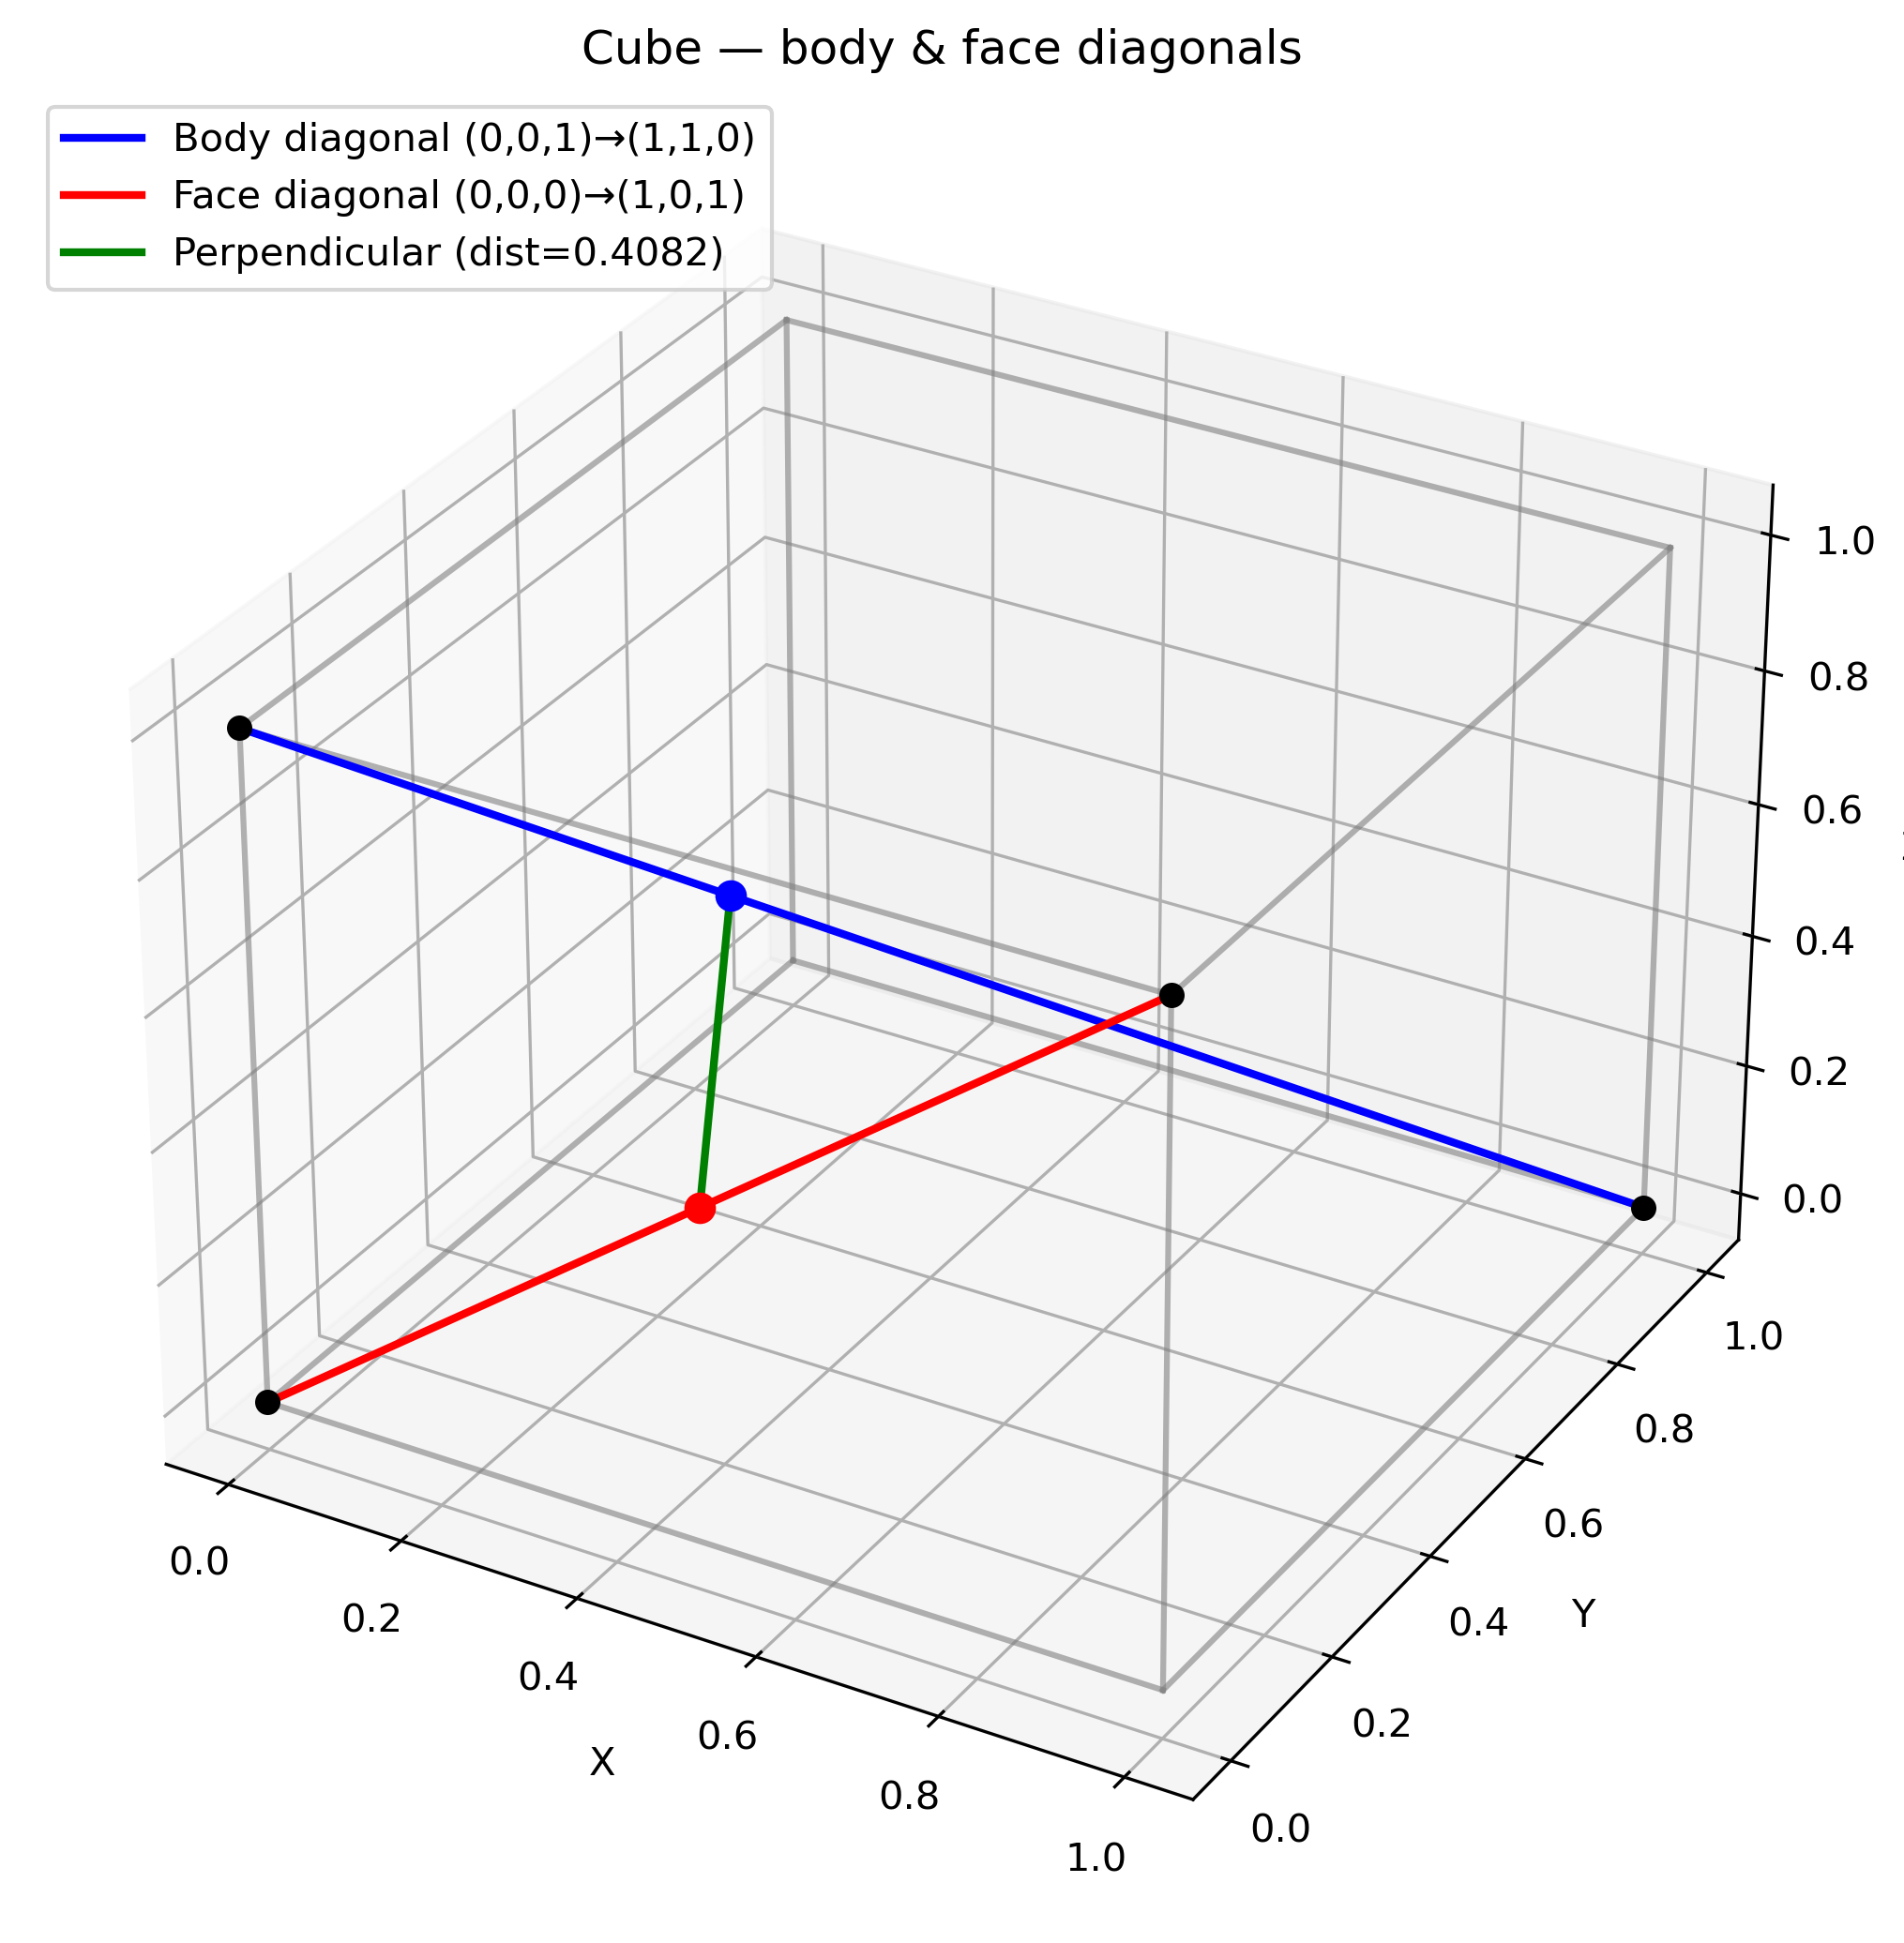
\includegraphics[width=0.7\columnwidth]{JEE/chapters/2.10.84/figs/cube_lines.png} 
   \caption{}
  \label{fig:2.10.84/Fig1}
\end{figure}


 \item Let $\vec{P}$ be the plane $3x + 2y + 3z = 16$ and let 
$$
S : \alpha \hat{i} + \beta \hat{j} + \gamma \hat{k}, \quad \text{where } \alpha + \beta + \gamma = 7
$$
and the distance of $(\alpha, \beta, \gamma)$ from the plane is $\frac{2}{\sqrt{22}}$.
Let $\vec{u}, \vec{v}, \vec{w}$ be three distinct vectors in $S$ such that $|\vec{u} - \vec{v}| = |\vec{v} - \vec{w}| = |\vec{w} - \vec{u}|$. Let $V$ be the volume of the parallelepiped determined by vectors $\vec{u}, \vec{v}, \vec{w}$. Then the value of $\frac{80}{3} V$ is
\rule{1cm}{0.1pt}.
\hfill (2023)
\item Let the position vectors of the points $\vec{P}, \vec{Q}, \vec{R},$ and $\vec{S}$ be
\begin{align*}
{\overrightarrow{a}} &= \hat{i} + 2\hat{j} - 5\hat{k}\\ {\overrightarrow{b}} &= 3\hat{i} + 6\hat{j} + 3\hat{k}\\ {\overrightarrow{c}} &= \frac{17}{5}\hat{i} + \frac{16}{5}\hat{j} + \frac{7}{5}\hat{k}\\ {\overrightarrow{d}} &= 2\hat{i} + \hat{j} + \hat{k}
\end{align*}
	respectively. Then which of the following statements is true?
\hfill (2023)
\begin{enumerate}
\item The points $\vec{P}, \vec{Q}, \vec{R},$ and $\vec{S}$ are NOT coplanar
\item $\frac{\vec{\overrightarrow{b}} + 2\vec{\overrightarrow{d}}}{3}$ is the position vector of a point which divides $PR$ internally in the ratio $5:4$
\item $\frac{\vec{\overrightarrow{b}} + 2\vec{\overrightarrow{d}}}{3}$ is the position vector of a point which divides $PR$ externally in the ratio $5:4$
\item The square of the magnitude of the vector $\vec{\overrightarrow{b}} \times \vec{\overrightarrow{d}}$ is $95$
\end{enumerate}
%
\item Let $\mathbb{R}^3$ denote the three-dimensional space. Take two points $\vec{P} = \brak{1,2,3}$ and $\vec{Q} = \brak{4,2,7}$. Let $dist\brak{\vec{X},\vec{Y}}$ denote the distance between two points $\vec{X}$ and $\vec{Y}$ in $\mathbb{R}^3$. Let  

\[
S = \{ \vec{X} \in \mathbb{R}^3 \; : \; \brak{dist\brak{\vec{X},\vec{P}}}^2 - \brak{dist\brak{\vec{X},\vec{Q}}}^2 = 50 \}
\]

\[
T = \{ \vec{Y} \in \mathbb{R}^3 \; : \; \brak{dist\brak{\vec{Y},\vec{Q}}}^2 - \brak{dist\brak{\vec{Y},\vec{P}}}^2 = 50 \}
\]

Then which of the following statements is {are} TRUE?
\hfill (2024)
\begin{enumerate}
\item There is a triangle whose area is $1$ and all of whose vertices are from $S$.
\item There are two distinct points $\vec{L}$ and $\vec{M}$ in $T$ such that each point on the line segment $LM$ is also in $T$.
\item There are infinitely many rectangles of perimeter $48$, two of whose vertices are from $S$ and the other two vertices are from $T$.
\item There is a square of perimeter $48$, two of whose vertices are from $S$ and the other two vertices are from $T$.
\end{enumerate}
\end{enumerate}

\item 
A line perpendicular to the line segment joining the points $\vec{P}(1, 0)$ and $\vec{Q}(2, 3)$ divides it in the ratio $1:n$. Find the equation of the line.
	\\
	\solution 
\label{chapters/11/10/2/11}
\begin{enumerate}[label=\thesection.\arabic*.,ref=\thesection.\theenumi]
\numberwithin{equation}{enumi}
\item The equation of a line is given by 
\begin{align}
			\label{eq:app-line-school}
	y &= mx + c
	\\
	\implies \myvec{x \\ y} &= \myvec{x \\ 
	 mx + c} =\myvec{0 \\ c} + x\myvec{1 \\ m}
\end{align}
			yielding \eqref{eq:geo-param}.
\item 			\eqref{eq:app-line-school} can also be expressed as
\begin{align}
	y - mx &= c 
	\\
	\implies \myvec{-m & 1}\myvec{x \\ y} &= c
\end{align}
			yielding \eqref{eq:geo-normal}.
		\item The direction vector is 
\begin{align}
			\label{eq:app-line-school-dir}
\vec{m} = \myvec{1 \\ m}
\end{align}
and the normal vector is
\begin{align}
\vec{n}=\myvec{-m \\ 1}
			\label{eq:app-line-school-normal}
\end{align}
  \item From \eqref{eq:geo-param}, 
	  if $\vec{A},\vec{D}$ and $\vec{C}$ are on the same line,
		\label{prop:app-lin-dep}
\begin{align}
			\vec{D}=\vec{A}+q\vec{m} 
			\\ 
			\vec{C}=\vec{D}+p\vec{m} \\
			\label{eq:app-collinear} 
			\implies 	p\brak{\vec{D}-\vec{A}} 
			+ q\brak{\vec{D}-\vec{C}} = 0, \quad p, q \ne 0 \\ 
			\implies \vec{D} = \frac{p\vec{A}+q\vec{C}}{p+q} 
			\end{align} 
			yielding \eqref{eq:section_formula} upon substituting \begin{align} k = \frac{p}{q}. \end{align} 
			$\brak{\vec{D}-\vec{A}}, \brak{\vec{D}-\vec{C}}$ 
		are then said to be {\em linearly dependent}.
	\item If $\vec{A}, \vec{B}, \vec{C}$ are collinear,  from \eqref{eq:geo-normal}, \begin{align}
	 \vec{n}^{\top}\vec{A} &=  c 
	 \\
	 \vec{n}^{\top}\vec{B} &=  c 
	 \\
	 \vec{n}^{\top}\vec{C} &=  c 
\end{align}
which can be expressed as 
\begin{align}
		\label{prop:app-lin-eq}
	\myvec{ \vec{A} & \vec{B} & \vec{C}}^{\top}\vec{n} = c\myvec{1 \\ 1 \\ 1}
	\\
	\equiv \myvec{ \vec{A} & \vec{B} & \vec{C}}^{\top}\vec{n} = \myvec{1 \\ 1 \\ 1}
		\label{prop:app-lin-eq-unit-mat},
	\\
	\implies 
	\myvec{ \vec{A} & \vec{B} & \vec{C}\\ 1 & 1 &1 }^{\top}\myvec{\vec{n} \\ -1} &= \vec{0}
		\label{prop:app-lin-dep-rank}
\end{align}
yielding
		\begin{align}
			\label{eq:app-line-rank-2}
			\rank{\myvec{1 & 1 & 1 \\ \vec{A}& \vec{B}&\vec{C}}} = 2
		\end{align}
			  Rank is defined to be the number of linearly indpendent rows or columns of a matrix.
		\item
The equation of a line can also be expressed as
\begin{align}
	 \vec{n}^{\top}\vec{x} &=   1
		\label{prop:app-lin-eq-unit}
\end{align}
	  \end{enumerate}

\item Find the vector equation of a plane which is at a distance of 7 units from the origin and normal to the vector $3\hat{i}+5\hat{j}-6\hat{k}$.
	\\
    \solution
		Let 
\begin{align}
	\vec{a} = \myvec{1\\1\\1} , \vec{b} = \myvec{2\\ -7 \\ -3}, 
\vec{c} = \myvec{\dfrac{1}{\sqrt{3}}\\[2ex] \dfrac{1}{\sqrt{3}} \\[2ex] -\dfrac{1}{\sqrt{3}}} 
\label{eq:chapters/12/10/2/1/1}
\end{align}
Then
\begin{align}
	{\vec{a}^{\top}\vec{a}} &= \myvec{1  &  1  &  1}\myvec{1\\1\\1} = 3
\\
\implies 
	\norm{\vec{a}}&=\sqrt{3}, 
	\label{eq:chapters/12/10/2/1/3}
\end{align}
		from \eqref{eq:side-length}. Similarly,
\begin{align}
	\norm{\vec{b}}&=\sqrt{\vec{b}^{\top}\vec{b}}= \sqrt{62}, 
	\label{eq:chapters/12/10/2/1/4}
	\\ \norm{\vec{c}}&=\sqrt{\vec{c}^{\top}\vec{c}}	
=1
	\label{eq:chapters/12/10/2/1/5}
\end{align}




\item Find the equation of a plane which is at a distance 3$\sqrt{3}$ units from origin and the normal to which is equally inclined to the coordinate axis.
\item If the line drawn from the point $(-2, -1, -3)$ meets a plane at right angle at the point $(1, -3, 3)$,  find the equation of the plane.
\item Find the equation of the plane through the points $(2, 1, -1)$ and $(-1, 3, 4), $ and 
perpendicular to the plane $x-2y+4z=10.$
\item If the foot of perpendicular drawn from the origin to a plane is $(5, -3, -2)$,  then the equation of the plane is $\overrightarrow{r} \cdot (5\hat{i}-3\hat{j}-2\hat{k})=38.$
\item  $\vec{P}(0, 2)$ is the point of intersection of $Y$ axis and perpendicular bisector of line segment joining the points $\vec{A}(-1, 1) \text{ and } \vec{B}(3, 3)$.
	\item The distance of the point $\vec{P}(2,  3)$ from the x-axis is
\rule{1cm}{0.1pt}.
\item Find the foot of perpendicular from the point $(2, 3, -8)$ to the line  
\begin{align*}
	\dfrac{4-x}{2}=\dfrac{y}{6}=\dfrac{1-z}{3}.
\end{align*}
	Also,  find the perpendicular distance from the given point to the line.
\item Find the distance of a point $(2, 4, -1)$ from the line $$\frac{x+5}{1}=\frac{y+3}{4}=\frac{z-6}{-9}.$$
\item Find the length and the foot of perpendicular from the point $ \brak{1, \dfrac{3}{2} , 2 }$ to the plane $2x-2y+4z+5=0.$
\item Show that the points $(\hat{i}-\hat{j}+3\hat{k})$ and $3(\hat{i}+\hat{j}+\hat{k})$ are equidistant from the plane $\overrightarrow{r} \cdot (5\hat{i}+2\hat{j}-7\hat{k})+9=0$ and lie on opposite side of it.
\item The distance of the plane $\overrightarrow{r} \cdot \brak{ \dfrac{2}{7}\hat{i}+\dfrac{3}{7}\hat{j}-\dfrac{6}{7}\hat{k}}=1$ from the origin is 
\rule{1cm}{0.1pt}.
\item The equation of the line passing through the point (1, 2) and perpendicular to the line $x+y+1=0$ is
\rule{1cm}{0.1pt}.
\item The equations of the lines passing through the point (1, 0) and at a distance $\frac{\sqrt{3}}{2}$ from the origin,  are 
\rule{1cm}{0.1pt}.
\item The foot of perpendiculars from the point (2, 3) on the line $y=3x+4$ is given by 
\rule{1cm}{0.1pt}.
\item A point equidistant from the lines $4x+3y+10=0$,  $5x-12y+26=0$ and $7x+24y-50=0$ is
\rule{1cm}{0.1pt}.
\item The ratio in which the line $3x+4y+2=0$ divides the distance between the lines $3x+4y+5=0$ and $3x+4y-5=0$ is
\rule{1cm}{0.1pt}.
\item Find the vector equation of the line passing through $(1, 2, 3)$ and perpendicular to the plane $\overrightarrow{r}\cdot(\hat{i}+2\hat{j}-5\hat{k})+9=0$ .
\item Find the equation of the plane passing through the point $(-1, 3, 2)$ and perpendicular to each of the planes $x+2y+3z=5$ and $3x+3y+z=0$.
\item If the points $(1, 1, p)$ and $(-3, 0, 1)$ be equidistant from the plane $\overrightarrow{r}\cdot(3\hat{i}+4\hat{j}-12\hat{k})+13=0$,  then find the value of $p$.
\item If $\vec{O}$ be the origin and the coordinates of $\vec{P}$ be $(1, 2, -3)$,  then find the equation of the plane passing through $\vec{P}$ and perpendicular to $OP$.
\item Find the vector equations of the line passing through the point $(1, 2, -4)$ and perpendicular to the two lines
$$\frac{x-8}{3}=\frac{y+19}{-16}=\frac{z-10}{7}\text{ and } \frac{x-15}{3}=\frac{y-29}{8}=\frac{z-5}{-5}.$$
\item Distance between the two planes: $2x+3y+4z=4$ and $4x+6y+8z=12$ is \label{prob:22}
\rule{1cm}{0.1pt}.
\item Find the equation of the line whose perpendicular distance from the origin is $4$ units and the angle which the normal makes with positive direction of x-axis is $15\degree$.
\item Find the distance of the point $(3, -5)$ from the line $3x-4y-26=0$.
\item Find the distance between the parallel lines $3x-4y+7=0$ and $3x-4y+5=0$.
\item Find the equation of a line perpendicular to the line $x+2y+3=0$ and passing through the point $(1, -2)$.
\item Reduce the equation $\sqrt3x+y-8=0$ into normal form. Find the values of $p$ and $\omega$.
\item Find the coordinates of the foot of the perpendicular drawn from the origin to the plane $2x -3y +4z -6 = 0$.
\item Find the equation of the plane which passes through the point $(5,  2,  -4)$ and perpendicular to the line with direction ratios $2,  3,  -1$.
\item Find the equation of the plane that contains the point $(1,  -1,  2)$ and is perpendicular to each of the planes $2x +3y -2z =5$ and $x +2y -3z =8$.
\item Find the distance between the point $\vec{P}(6,  5,  9)$ and the plane determined by the points $\vec{A}(3,  -1, 2),  \vec{B}( 5,  2, 4)$ and $\vec{C}(-1,  -1,  6)$.
\item Find the distance of a point $(2,  5,  -3)$ from the plane $\overrightarrow{r} \cdot (6\hat{i} -3\hat{j} +2\hat{k}) =4$.
\item A line passes through (2, 2) and is perpendicular to the line $3x+y=3$. Its $y$-intercept is 
\rule{1cm}{0.1pt}.
		
\end{enumerate}
